\chapter{Preliminaries}
\label{cha:prelim}

% \TODO{change after revision}
In this chapter, we start with the notations used in this thesis~\autoref{sec:notations}. Afterwards, we describe the basic knowledge of secure multi-party computation in~\autoref{sec:secureMultipartyComputation}. Finally, we introduce the background knowledge and theory of differential privacy in~\autoref{sec:differentialPrivacy}.

\section{Notations}
\label{sec:notations}

% \CHANGED{revised based on feedback}

% For $a,b,c \in \mathbb{N} $, let $\left[a\right] $ denote $\left\{x\in \mathbb{Z} \,|\, 1 \leq x \leq a\right\} $, $\left(a,b\right) $ is $\left\{x\in \mathbb{R} \, | \, a<x< b\right\} $, and $\left[a,b\right] $ is $\left\{x\in \mathbb{R} \, | \,a\leq x\leq b\right\} $. $\left\{a,b,c\right\} $ is a set containing the three numbers, and $\left(a_i\right)_{i \in \left[ n\right]}=\left(a_1,\ldots,a_n\right) $ is a sequence of $n$ numbers.
For $a,b,c \in \mathbb{N} $, $\left(a,b\right) $ denotes $\left\{x\in \mathbb{R} \, | \, a<x< b\right\} $, and $\left[a,b\right] $ denotes $\left\{x\in \mathbb{R} \, | \,a\leq x\leq b\right\} $. $\left\{a,b,c\right\} $ is a set containing the three numbers.
$\mathbb{D}$ denotes the set of floating-point numbers, and $\mathbb{D} \cap \left(a,b\right) $ contains floating-point numbers in the interval $\left(a,b\right)$.

Let $P_1, \ldots P_{N} $ denote $N$ computation parties. The value $x$ that is secret shared among $N$ parties are denoted by $\left\langle x\right\rangle ^{S,D}=\left(\left\langle x\right\rangle_1^{S,D} ,\ldots, \left\langle x\right\rangle_N^{S,D}\right) $, where
$\left\langle x\right\rangle _i^{S,D}$ is hold by party $P_i$.
Superscript $S \in \left\{\ARITH,\BOOL,\YAO\right\} $ denotes the sharing type (cf.~\autoref{subsec:MPCProtocols}): \ARITH for arithmetic sharing, \BOOL for Boolean sharing with GMW, \YAO for Yao sharing with BMR.
% $\operatorname{B2A}$ denotes the share conversion from $\BOOL$ to $\ARITH$, and other share conversions are defined similarly as discussed in~\cite{demmler2015aby}.
Superscript $D \in \left\{\uint,\sint,\fx,\fl \right\} $ indicates the data type: \uint for unsigned integer, \sint for signed integer, \fx for fixed-point number, and \fl for floating-point number. We omit subscript and subscript when it is clear from the context.

The bold symbol $\left\langle \boldsymbol{x}\right\rangle $ denotes a vector of $\ell$ shared bits.
We use $\operatorname{XOR}$ ($\oplus $), $\operatorname{AND}$ ($\land $), and $\operatorname{NOT}$ ($\neg$) in the logical operations.
Let $\left\langle {a}\right\rangle^{S,D} \odot \left\langle {b}\right\rangle^{S,D}$ be the arithmetic operations on two shared numbers, where $\odot\in\left\{+, -, \cdot, \div, >, ==\right\} $. $\left\langle a\right\rangle ^{\BOOL} \cdot \left\langle \boldsymbol{b}\right\rangle ^{\BOOL}$ represents the bitwise $\operatorname{AND}$ operations between $\left\langle a\right\rangle ^{\BOOL}$ and every Boolean sharing bit $\left\langle b\right\rangle^{\BOOL} \in\left\langle \boldsymbol{b}\right\rangle ^{\BOOL}$.
% Other arithmetic operations are defined similarily.
% Similarly, $\ln\left(\left\langle {a}\right\rangle \right) $, $2^{\left\langle {a}\right\rangle } $, $e^{\left\langle {a}\right\rangle^{D} }$, $\left\lvert \left\langle {a}\right\rangle^{D} \right\rvert $, $\left\lfloor \left\langle {a}\right\rangle^{D} \right\rfloor $ , $\left\lceil \left\langle {a}\right\rangle^{D} \right\rceil $, $\left\langle {a}\right\rangle^{D} \mod \left\langle {b}\right\rangle^{D} $ denote the arithmetic operations of shared numbers $\left\langle {a}\right\rangle^{D} $ and $\left\langle {b}\right\rangle^{D} $ of type $D$.
Let $\left\langle {a}\right\rangle ^{\fl}=\Uppi^{UINT2FL}\left(\left\langle {a}\right\rangle ^{\uint}\right) $ be the conversion from a shared unsigned integer $\left\langle {a}\right\rangle ^{\uint}$ to a shared floating-point number $\left\langle {a}\right\rangle ^{\fl}$. Other data type conversion operations are defined in a similar manner.


\section{Secure Multi-Party Computation (SMPC)}
\label{sec:secureMultipartyComputation}
Secure Multi-Party Computation enables multiply parties to jointly evaluate a function on their private inputs while revealing only the computation result. Yao~\cite{yao1982protocols} introduced the concept of secure two-party computation with Yao's Millionaires' problem (i.e., two millionaires wish to know who is richer without revealing their actual wealth) and proposed the Yao's Grbled Circuit protocol~\cite{yao1986generate} as a solution.
In the Yao's Grbled Circuit protocol, the target function is represented as a Boolean circuit consisting of connected gates and wires. One party called gabler is responsible for garbling the circuit, and the other party called evaluator evaluates the garbled circuit and outputs the result.
% The gabler generates the garbled circuit by replacing the logical values ($0$ and $1$) of each wire with two random keys. Then, the gabler encrypted and shuffle the truth table of each gate with these keys. 

% In Yao's Millionaires' problem, two millionaires wish to know who is richer without revealing their actual wealth.
Afterwards, \bmr~\cite{beaver1990round} generalized Yao's Garbled Circuit protocol~\cite{yao1986generate} to multi-party settings. \gmw~\cite{goldreich1987play} proposed a general solution to \smpc based on secret sharing, where each party splits his data into several shares and sends it to each of the parties.
Secret sharing guarantees that any secret shares held by a single party leak no information about the parties' private input.

Generally, the execution of \smpc protocols is separated into two phases: an offline (or preprocessing) phase and an online phase.
In the offline phase, the parties compute everything that does not depend on the private input. In the online phase, the parties compute the input-dependent part.


\subsection{Security Model}
\label{subsec:SecurityModel}
The standard approach to prove the security of cryptographic protocols is to consider adversaries with different capabilities.
We describe two types of adversaries: the \textit{semi-honest} adversary and the \textit{malicious} adversary. We refer to~\cite[Chapter~2]{evans2017pragmatic} for a formal and detailed description of the security model.

\textbf{Semi-honest adversaries} (also known as passive adversaries) try to infer additional information about other parties from the messages during the protocol execution without attempting to break the protocol. Therefore, it is a weak security model and only prevents the unintentional disclosure of information between parties. The semi-honest protocols are usually very efficient and the first step to design protocols with stronger security guarantees.

\textbf{Malicious adversaries} (also known as active adversaries) may cause corrupted parties to arbitrarily deviate from the protocol specification and attempt to learn information about the other parties' inputs. Protocols against malicious adversaries usually deploy cryptographic mechanisms to ensure that the parties cannot deviate from the protocol specification. Therefore, it is often more expensive than the protocol against semi-honest adversaries.

\subsection{Cryptographic Primitives}
\label{subsec:CryptographicPrimitivesforSecureMulti-PartyComputation}

\subsubsection{Oblivious Transfer}
\label{subsubsec:OT}
% \ot was first defined by Rabin~\cite{rabin2005exchange} as a mode of transferring information, where the receiver $P_R$ received the message from the sender $P_S$ successfully with probability $p=0.5$, and the sender was oblivious of whether the message was received.
% Later, Even et al.~\cite{even1985randomized} redefined OT as the $1$-out-of-$2$ OT ($\binom{2}{1}$-OT). $\binom{2}{1}$-OT has the functionality that accepts inputs ($x_0$, $x_1$) from the sender and a choice bit $c$ from the receiver. After computation, it outputs $\bot $ to the sender and $x_c$ to the receiver. $\binom{2}{1}$-OT guarantees that the sender does not learn anything about $c$ and the receiver does not learn about $x_{1-c}$.
% Impagliazzo and Rudich~\cite{impagliazzo1989limits} showed that a \textit{black-box} reduction from OT to a one-way function~\cite[Chapter~2]{oded2006foundations} is as hard as proving $P\neq NP$, which implies that OT requires relatively expensive (than symmetric cryptography) public-key cryptography~\cite{rivest1978method}.

\ot is a cryptographic primitive that enables two parties to obliviously transfer one value out of two values. Specifically, the sender has inputs ($x_0$, $x_1$), and the receiver has a choice bit $c$. Oblivious transfer protocol receives the inputs from the sender and receiver, and outputs $x_c$ to the receiver. It guarantees that the sender does not learn anything about $c$ and the receiver does not learn about $x_{1-c}$.
Impagliazzo and Rudich~\cite{impagliazzo1989limits} showed that a \textit{black-box} reduction from \ot to a one-way function~\cite[Chapter~2]{oded2006foundations} is as hard as proving $P\neq NP$, which implies that \ot requires relatively expensive (than symmetric cryptography) public-key cryptography~\cite{rivest1978method}.

Nevertheless, Ishai et al.~\cite{ishai2003extending} proposed \ot \textit{extension} techniques that extend a small number of OTs based on public-key cryptography to a large number of OTs with efficient symmetric cryptography.
Asharov et al.~\cite{asharov2017more} proposed specific \ot functionalities for the optimization of \smpc protocols, such as \correlatedot and \randomot. In \correlatedot, the sender inputs a correlation function $f_{\Delta }$ (e.g., $f_{\Delta }\left(x\right)=x\oplus \Delta $, where $\Delta$ is only known by the sender) and receives random values $x_0$ and $x_1=f_{\Delta }\left(x_0\right)$. The receiver inputs a choice bit $c$ and receives $x_{c}$. In \randomot, the sender has no inputs and receives random values ($x_0$, $x_1$), and the receiver inputs a choice bit $c$ and receives $x_c$.

\subsubsection{Multiplication Triples}
\label{subsubsec:MTs}
\mts were proposed by Beaver~\cite{beaver1991efficient} that can be precomputed to reduce the online complexity of \smpc protocols by converting expensive operations (e.g., arithmetic multiplication and logical $\operatorname{AND}$) to linear operations (e.g., arithmetic addition and logical $\operatorname{XOR}$).

A multiplication triple has the form $\left(\left\langle a\right\rangle^S , \left\langle b\right\rangle^S,\left\langle c\right\rangle^S\right) $ with $S\in \left\{B,A\right\} $.
We have $c=a\land b$ for Boolean sharing (cf.~\autoref{subsubsec:BooleanSharingwithGMW}) and $c=a \cdot  b$ for arithmetic sharing (cf.~\autoref{subsubsec:ArithmeticSharing}).
Multiplication triples can be generated using \correlatedot (cf.~\autoref{subsubsec:OT}) in the two-party setting~\cite{demmler2015aby} or in the multi-party setting~\cite{braun2022motion}.
% The advantage of \mts is that it can reduce the MPC protocols' online complexity by converting expensive operations (e.g., arithmetic multiplication and logical $\operatorname{AND}$) to linear operations (e.g., arithmetic addition and logical $\operatorname{XOR}$).


% \subsection{Yao's Garbled Circuit Protocol}
% \label{subsec:YaoGarbledCircuitProtocol}

\subsection{MPC Protocols}
\label{subsec:MPCProtocols}
We describe the \smpc protocols that are secure against $N-1$ semi-honest corruptions: Arithmetic sharing (cf.~\autoref{subsubsec:ArithmeticSharing}), Boolean sharing with \gmw (cf.~\autoref{subsubsec:BooleanSharingwithGMW}), and Yao sharing with \bmr (cf.~\autoref{subsubsec:YaoSharingwithBMR}).
We refer to~\cite{demmler2015aby, braun2022motion} for a formal and detailed description.

\subsubsection{Arithmetic Sharing (\ARITH)}
\label{subsubsec:ArithmeticSharing}
The arithmetic sharing protocol enables parties to evaluate arithmetic circuits consisting of addition and multiplication gates.
In arithmetic sharing, an $\ell$-bit value $x$ is shared additively among $N$ parties as $\left(\left\langle x\right\rangle ^A_1, \ldots,\left\langle x\right\rangle ^A_N \right) \in \mathbb{Z} ^N_{2^{\ell}}$, where $x=\sum_{i=1}^{N} \left\langle x\right\rangle^A_i \mod{2^{\ell}} $ and party $P_i$ holds $\left\langle x\right\rangle^A_i $. Value $x$ can be reconstructed by letting each party $P_i$ sends $\left\langle x\right\rangle^A_i $ to one specific party who computes $x=\sum_{i=1}^{N} \left\langle x\right\rangle^A_i \mod{2^{\ell}}$.
The addition of arithmetic shares can be computed without parties' interaction. Suppose the parties hold shares $\left\langle x\right\rangle^A_i $, $\left\langle y\right\rangle^A_i $, and wish to compute $\left\langle z\right\rangle =a \cdot \left\langle x\right\rangle +\left\langle y\right\rangle +b$ with public value $a$, $b\in \mathbb{Z} _{2^{\ell}}$. Then, one specific party $P_1$ computes $\left\langle z\right\rangle ^A_1=a \cdot \left\langle x\right\rangle^A_1 +\left\langle y\right\rangle^A_1 +b$, and the other parties compute $ \left\langle z\right\rangle ^A_i=a \cdot \left\langle x\right\rangle^A_i +\left\langle y\right\rangle^A_i $ locally.

The multiplication of arithmetic shares can be performed using \mts (cf.~\autoref{subsubsec:MTs}). Suppose $\left(\left\langle a\right\rangle^A ,\left\langle b\right\rangle^A,\left\langle c\right\rangle^A\right) $ is an \mts in $\mathbb{Z} _{2^{\ell}}$, where $c =a \cdot b $. To compute $\left\langle z\right\rangle ^A = \left\langle x\right\rangle ^A \cdot \left\langle y\right\rangle ^A$, the parties first locally compute $\left\langle d\right\rangle ^A_i=\left\langle x\right\rangle ^A_i-\left\langle a\right\rangle^A_i $ and $\left\langle e\right\rangle ^A_i=\left\langle y\right\rangle ^A_i-\left\langle b\right\rangle ^A_i$, and reconstruct them to get $d$ and $e$. Finally, the parties compute $\left\langle z\right\rangle ^A = \left\langle c\right\rangle ^A+e \cdot \left\langle x\right\rangle ^A+d \cdot \left\langle y\right\rangle ^A- d \cdot e$.

\subsubsection{Boolean Sharing with GMW}
\label{subsubsec:BooleanSharingwithGMW}
Boolean \gmw protocol~\cite{goldreich1987play} uses $\operatorname{XOR}$-based secret sharing and enables multiple parties to evaluate the function represented as a Boolean circuit. A bit $x\in\left\{0,1\right\} $ is shared among $N$ parties as $\left(\left\langle x\right\rangle ^B_1, \ldots,\left\langle x\right\rangle ^B_N \right) \in \left\{0,1\right\}^N$, where $x=\bigoplus _{i=1}^N \left\langle x\right\rangle ^B_i$. Boolean \gmw can be seen as a special case of arithmetic sharing protocol. Operation $\left\langle x\right\rangle^B_i \oplus  \left\langle y\right\rangle^B_i $ and $\left\langle x\right\rangle^B_i \land\left\langle y\right\rangle^B_i$ are computed analogously as in the arithmetic sharing.
% \paragraph{Boolean Sharing with GMW (B)}
% \label{para:BooleanSharing}

\subsubsection{Yao Sharing with BMR}
\label{subsubsec:YaoSharingwithBMR}

% We describe a generic case of GMW protocol where two parties $P_0$ and $P_1$ wish to securely evaluate a Boolean circuit $C$.
% Each party first secret shares its input bits with other parties using an $\operatorname{XOR}$-based secret sharing scheme. For example, $P_{0}$ has input bit $x$ and sends its share $x_{1} $ to $P_1$, where $x=x_0 \oplus x_1$. $P_1$ with input bit $y$ follows the same secret sharing steps.
% The $\operatorname{XOR}$ gate $z=x\oplus y$ can be evaluated by each party $P_i$ locally with $z_i= x_i \oplus y_i$ since $z= x\oplus y = \left(x_0 \oplus x_1\right) \oplus \left(y_0 \oplus y_1\right) =\left(x_0 \oplus y_0\right) \oplus \left(x_1 \oplus y_1\right)$.

% We describe the steps to evaluate an $\operatorname{AND}$ gate $z=x \land y$ using OT (cf.~\autoref{subsubsec:OT}).
% Other techniques such as Multiplication Triple~\cite{beaver1991efficient} can also be applied for the evaluation.

% \subsubsection{Evaluation of AND Gate with OT~\cite{choi2012secure, zohner2017faster}}
% $P_0$ acts as the sender of a $\binom{4}{1} $-OT with inputs $\left(s_0,s_1,s_2,s_3\right) $ that is calculated with his shared bits $x_0$, received bits $y_0$, and a random bit $z_0$ as follows:

% \begin{equation}
%     \begin{split}
%         s_0=& z_{0} \oplus\left(\left(x_{0}\oplus 0 \right) \land \left(y_{0}\oplus 0\right) \right) \\
%         s_{1}= & z_{0} \oplus\left(\left(x_{0}\oplus 0\right)  \land\left(y_{0} \oplus 1\right)\right) \\
%         s_{2}= & z_{0} \oplus\left(\left(x_{0} \oplus 1\right) \land \left(y_{0}\oplus 0\right) \right) \\
%         s_{3}=&z_{0} \oplus\left(\left(x_{0} \oplus 1\right) \land\left(y_{0} \oplus 1\right)\right) .
%     \end{split}
% \end{equation}
% $P_1$ acts as the receiver with choice $\left(x_1y_1\right)_2 $ and receives $z_1=s_{\left(x_1y_1\right)_2 }=z_0\oplus \left(\left(x_0\oplus x_1\right)  \land \left(y_0\oplus  y_1\right)  \right)$. It is easy to verify that $z=z_0 \oplus z_1 $.



% \subsection{Beaver-Micali-Rogaway (\bmr)}
% \label{subsec:BMR}

We first present Yao's Garbled Circuit protocol~\cite{yao1986generate} following the steps described in work~\cite{lindell2009proof} and then extend it to multi-party settings with the \bmr~\cite{beaver1990round} protocol.
Yao's Garbled Circuit protocol~\cite{yao1986generate} enables two parties, the garbler, and the evaluator, to securely evaluate any functionality represented as a Boolean circuit.
% \subsubsection{Execution of Garbled Circuit Protocol}
% We : circuit garbling, input encoding, and circuit evaluation.

\textbf{1. Circuit Garbling.}
The garbler converts the jointly decided function $f$ into a Boolean circuit $C$, and selects a pair of random $\kappa$-bit keys $\left(k_0^i,k_1^i\right)\in \left\{0,1\right\}^{2\kappa}$ to represent logical value $0$ and $1$ for each wire. For each gate $g$ in the Boolean circuit $C$ with input wire $a$ and $b$, and output wire $c$, the gabler uses the generated random keys $\left(k_0^a,k_1^a\right)$, $\left(k_0^b,k_1^b\right)$, $\left(k_0^c,k_1^c\right)$ to create a garbled table $\tilde{g}$ based on the function table of $g$. For example, gate $g$ is an $\operatorname{AND}$ gate and has a function table as~\autoref{tabular:andGate} shows, the gabler encrypts the keys of wire $c$ and permutes the entries to generate ~\autoref{tabular:garbledAndGate}. Note that the symmetric encryption function $\operatorname{Enc}_k$ uses a secret-key $k$ to encrypt the plaintext, and its decryption function $\operatorname{Dec}_k$ decrypts the ciphertext successfully only when the identical secret-key $k$ is given. When all the gates in Boolean circuit $C$ are garbled, the gabler sends the garbled circuit $\widetilde{C}$ that consists of garbled tables from all the gates to the evaluator for evaluation.

\begin{table}[htbp]
    \centering
    \begin{tabular}{|c|c||c|}

        a            & b & c \\
        \hline     0 & 0 & 0 \\
        0            & 1 & 0 \\
        1            & 0 & 0 \\
        1            & 1 & 1 \\
    \end{tabular}
    \caption{Function table of $\operatorname{AND}$ gate $g$.}
    \label{tabular:andGate}
\end{table}

% \begin{table}[htbp]
%     \centering
%     \begin{tabular}{|c|c||c|}
%         $\tilde{a}$ & $\tilde{b}$ & $\tilde{c}$                                           \\
%         \hline
%         $k_1^a$     & $k_1^b$     & $\operatorname{Enc}_{k_1^a, k_1^b}\left(k_1^c\right)$ \\
%         $k_0^a$     & $k_1^b$     & $\operatorname{Enc}_{k_0^a, k_1^b}\left(k_0^c\right)$ \\
%         $k_0^a$     & $k_0^b$     & $\operatorname{Enc}_{k_0^a, k_0^b}\left(k_0^c\right)$ \\
%         $k_1^a$     & $k_0^b$     & $\operatorname{Enc}_{k_1^a, k_0^b}\left(k_0^c\right)$ \\
%     \end{tabular}
%     \caption{Garbled table of $\operatorname{AND}$ gate $g$ with encrypted and permuted entries.}
%     \label{tabular:garbledAndGate}
% \end{table}

\begin{table}[htbp]
    \centering
    \begin{tabular}{|c|c||c|}
        $\tilde{c}$                                           \\
        \hline
        $\operatorname{Enc}_{k_1^a, k_1^b}\left(k_1^c\right)$ \\
        $\operatorname{Enc}_{k_0^a, k_1^b}\left(k_0^c\right)$ \\
        $\operatorname{Enc}_{k_0^a, k_0^b}\left(k_0^c\right)$ \\
        $\operatorname{Enc}_{k_1^a, k_0^b}\left(k_0^c\right)$ \\
    \end{tabular}
    \caption{Garbled table of $\operatorname{AND}$ gate $g$ with encrypted and permuted entries.}
    \label{tabular:garbledAndGate}
\end{table}

\textbf{2. Input Encoding.}
The gabler sends the wire keys corresponding to his input directly to the evaluator. To evaluate the garbled circuit $\widetilde{C}$, the evaluator needs the wire keys corresponding to his input. For each of the evaluator's input wire $i$ with corresponding input bit $c$, the evaluator and the gabler run an $1$-out-of-$2$-OT, where the gabler acts as a sender with inputs $\left(k_0^i,k_1^i\right)$, and the evaluator acts as a receiver with input $c$ and receives $k_c^i$. Recall that \ot (cf.~\autoref{subsubsec:OT}) guarantees that the gabler learns nothing about $c$ and the evaluator learns only $k_{c}^i$.

\textbf{3. Circuit Evaluation.}
After receiving the garbled circuit $\widetilde{C}$ and the keys of input wires, the evaluator begins to evaluate the garbled circuit $\widetilde{C}$. For each gate $g$ with input wire $a$ and $b$, output wire $c$, the evaluator uses the input wire keys $\left(k^a,k^b\right)$ to decrypt the output key $k^c$. When all the gates in the garbled circuit $\widetilde{C}$ are evaluated, the evaluator obtains the keys for the output wires. To reconstruct the output, either the gabler sends the mapping from output wire keys to plaintext bits to the evaluator, or the evaluator sends the decrypted output wire keys to the gabler.


\paragraph{Optimizations for Yao's Garbled Circuits.}
\label{para:OptimizationsforYaosGarbledCircuits}
This part presents several prominent optimizations for Yao's Garbled Circuit protocol~\cite{yao1986generate}.
Recall that in the evaluation step of Yao's garbled circuit $\widetilde{C}$ protocol, the evaluator needs to decrypt at most four entries to obtain the correct key of the output wire. Point and permute~\cite{beaver1990round} technique helps the evaluator to identify the entry that should be decrypted in garbled tables with an additional permutation bit for each wire.
Garbled row reduction~\cite{naor1999privacy} reduces the number of entries in the garbled table from four to three by fixing the first entry to a constant value.
Free-XOR~\cite{kolesnikov2008improved} allows the parties to evaluate $\operatorname{XOR}$ gates without interactions by choosing all the wire key pairs $\left(k_0^i,k_1^i\right)$ with the same fixed distance $R$ ($R$ is kept secret to the evaluator), e.g., $k_0^i$ is chosen at random and $ k_1^i $ is set to $R\oplus k_0^i $.
Fixed-Key AES garbling~\cite{bellare2013efficient} reduces the encryption and decryption workload of Yao's Garbled Circuit protocol~\cite{yao1986generate} using a block cipher with a fixed key such that the AES key schedule is executed only once.
Two-halves garbling~\cite{zahur2015two} reduces the entry number of each $\operatorname{AND}$ gate from three to two by splitting each $\operatorname{AND}$ gate into two half-gates at the cost of one more decryption operation of the evaluator.
Three-halves garbling~\cite{rosulek2021three} requires $25\%$ less communication bits than the two-halves garbling at the cost of more computation.

\paragraph{BMR Protocol.}
\label{para:BMRProtocol}
The \bmr protocol~\cite{beaver1990round} extends Yao's Garbled Circuit protocol~\cite{yao1986generate} to multi-party settings. Recall that in Yao's Garbled Circuit protocol, the circuit is garbled by one party and evaluated by another party. At a high level, the \bmr protocol enables the multi-party computation by having all parties jointly garbling the circuit in the offline phase. Then, each party sends the garbled labels that are associated with their private inputs to other parties. Next, each party plays the role of the evaluator and evaluates the garbled circuit locally. Finally, the parties use the received garbled label and the result of local evaluation to reveal the output.


% \subsection{Secret Sharing and Sharing Conversions}
% \label{subsec:secretSharingAndSharingConversions}
% We introduce the secret sharing types and sharing conversions used based on work~\cite{demmler2015aby}.

% % \subsubsection{Secret Sharing}





% \paragraph{Yao Sharing with BMR (Y)}
% \label{para:YaoSharing}
% Recall that in Yao's garbled circuit protocol (cf.~\autoref{subsec:BMR}), we introduce the optimization techniques such as point and permute~\cite{beaver1990round} and Free-XOR~\cite{kolesnikov2008improved}. Specifically, the garbler generates a random $\kappa$-bit string $R$ with $R\left[0\right] =1$ (as permutation bit) and a random key $k_0^i$, and set $k_1^i=k_0^i\oplus R$ for each wire $i$.
% Based on the above techniques, the evaluator can share a bit $x$ with the garbler by running a C-OT (cf.~\autoref{subsubsec:OT}). The garbler inputs a correlation function $f_{R }$, obtains $\left(k_0,k_1 \right) $ with $k_1=k_0\oplus R$, and set $\left\langle x\right\rangle^Y_0 =k_0$. The evaluator inputs a choice bit $x$, and receives $\left\langle x\right\rangle^Y_1 =k_x=k_0\oplus x R$. To reconstruct $x$, the evaluator sends $\left\langle x\right\rangle^Y_1\left[0\right] $ to the garbler who computes $x=\left\langle x\right\rangle^Y_0\left[0\right]\oplus \left\langle x\right\rangle^Y_1\left[0\right]$.
% For the evaluation of $\operatorname{XOR}$ gate, each party can locally calculate $\left\langle z\right\rangle ^Y=\left\langle x\right\rangle^Y\oplus \left\langle y\right\rangle ^Y $ based on Free-XOR~\cite{kolesnikov2008improved}. The $\operatorname{AND}$ gate $\left\langle z\right\rangle ^Y=\left\langle x\right\rangle^Y \land\left\langle y\right\rangle ^Y $ can be evaluated using the method from~\cite{bellare2013efficient}, where one party garbles the circuit with its share and another party evalutes the garbled circuit with its share.
% Yao's sharing can also be extended to multi-party case as the work~\cite{braun2022motion} showed.

% \subsubsection{Sharing Conversions}
% \label{subsubsec:SharingConversions}
% Different sharing types and corresponding MPC protocols have advantages in specific operations, e.g., arithmetic GMW (cf.~\autoref{subsec:GMW}) allows parties to execute linear operations locally, and BMR (cf.~\autoref{subsec:BMR}) is often more efficient for comparison. Therefore, we consider the sharing conversion methods introduced in works~\cite{demmler2015aby,braun2022motion}.

\subsection{SMPC Framework - MOTION}
\label{subsection:MOTIONFramework}
We build upon the MOTION~\cite{braun2022motion} framework that provides the following novel features:
\begin{enumerate}
    \item Support for \smpc with $N$ parties, full-threshold security (i.e., tolerating up to $N-1$ passive corruptions) and sharing conversions between $\left\{A,B,Y\right\} $.
    \item Implementation of primitive operations of \smpc protocols at the circuit's gate level and asynchronously evaluation, i.e., each gate is separately evaluated once their parent gates become ready.
    \item Support for \simd, i.e., vectors of data are processed instead of single data, that can reduce memory footprint and communication.
    \item Integration of HyCC compiler~\cite{buscher2018hycc} that can generate efficient circuits for hybrid MPC protocols with functionality described in C programming language.
\end{enumerate}
% We build our \smpc protocols primarily with Boolean \gmw (\BOOL) and arithmetic \gmw (\ARITH).


\section{Differential Privacy}
\label{sec:differentialPrivacy}
This section describes the concept of differential privacy in a formal mathematical view. We first introduce basic knowledge of probability distribution and random variable generation methods. Then, we describe traditional privacy preservation techniques and discuss their limitations. Next, we describe the motivation behind differential privacy and formalize its definition. Finally, we describe the differentially private mechanisms for realizing differential privacy.

\subsection{Probability Distribution and Random Variable Generation}
\label{subsec:probabilityDistribution}
In this section, we introduce essential probability theory and random variable sampling methods as a preparation for differential privacy.

\subsubsection{Continuous Probability Distribution}
\label{subsubsec:ContinuousProbabilityDistribution}

\begin{definition}[Continuous Uniform Distribution]
    \label{def:UniformDistribution}
    The continuous uniform distribution with two boundary parameters $a$ and $b$, has the following probability density function:
    \begin{equation}
        \begin{split}
            Uni\left(x \,|\,a,b\right)
            &=
            \begin{cases}
                \frac{1}{b-a} & \textit{ for } a\leq x\leq b \\
                0             & \textit{otherwise}
            \end{cases}
        \end{split}
    \end{equation}
\end{definition}

We use the probability density function to denote the corresponding probability distribution or a random variable sampled from that distribution. For example, $Uni\left(a,b\right)$ denotes the continuous uniform distribution with parameters $a$ and $b$. We sometimes abuse notation and let $Uni\left( a,b\right)$ denote a random variable $x \sim Uni\left( a,b\right)$.


\begin{definition}[Exponential Distribution]
    \label{def:ExponentialDistribution}
    The exponential distribution with rate parameter $\lambda>0$ has the following probability density function:
    \begin{equation}
        \begin{split}
            Exp\left(x \,|\,\lambda\right)            &=
            \begin{cases}
                \lambda e^{-\lambda x } & \textit{ for }  x\geq 0 \\
                0                       & \textit{ for }  x <0
            \end{cases}
        \end{split}
    \end{equation}
\end{definition}
% $Exp\left(\lambda\right)$ denotes the exponential distribution with parameter $\lambda$.
The cumulative distribution function of an exponential distribution is defined as:
\begin{equation}
    \begin{split}
        \Pr\left( x\,|\,\lambda\right)=
        \begin{cases}
            1- e^{-\lambda x} & \textit{ for } x \geq 0 \\
            0                 & \textit{ for } x < 0    \\
        \end{cases}
    \end{split}
\end{equation}


\begin{definition}[Laplace Distribution{~\cite{dwork2014algorithmic}}]
    \label{def:LaplaceDistribution}
    The Laplace distribution (centered at $0$) with scale parameter $b$, has the following probability density function:
    \begin{equation}
        \begin{split}
            Lap\left(x \,|\,b\right)&= \frac{1}{2b}e^{\left( -\frac{\left| x\right| }{b}\right)}
        \end{split}
    \end{equation}
\end{definition}
The Laplace distribution is a symmetric version of the exponential distribution. It is also called the double exponential distribution because it can be considered as an exponential distribution assigned with a randomly chosen sign.
% We write $Lap\left(b\right)$ to denote the Laplace distribution with scale parameter $b$ and $x \sim Lap\left( b\right)$ to denote a Laplace random variable.

The cumulative distribution function of the Laplace distribution is defined as:
\begin{equation}
    \Pr\left( x\leq X\,|\,b\right)=
    \begin{cases}
        \frac{1}{2} e^{\frac{X}{b}}     & \textit{ for } X \leq 0 \\
        1- \frac{1}{2} e^{-\frac{X}{b}} & \textit{ for } X > 0    \\
    \end{cases}
\end{equation}


\begin{definition}[Gaussian Distribution]
    \label{def:GaussianDistribution}
    The univariate Gaussian (also known as the standard normal) distribution with mean $\mu$ and standard deviation $\sigma$, has the following probability density function:
    \begin{equation}
        \begin{split}
            \mathcal{N} \left( x \,|\, \mu,\sigma\right)&=\frac{1}{\sigma\sqrt{2 \pi}}e^{-\frac{1}{2}\left( \frac{x-\mu}{\sigma}\right) ^{2}}
        \end{split}
    \end{equation}
\end{definition}
% $\mathcal{N} \left( \mu,\sigma\right)$ denotes the Gaussian distribution with mean $\mu$ and standard deviation $\sigma$.
% $x \sim \mathcal{N}  \left(\mu,\sigma\right)$ is a Gaussian random variable.


\subsubsection{Discrete Probability Distribution}
\label{subsubsec:DiscreteProbabilityDistribution}

\begin{definition}[Bernoulli distribution]
    \label{def:BernoulliDistribution}
    The Bernoulli distribution with parameter $p \in \left[0,1\right] $ has the following probability mass function:
    \begin{equation}
        \begin{split}
            Bern\left(x \,|\,p \right)&=
            \begin{cases}
                p   & \textit{ for } x =1 \\
                1-p & \textit{ for } x =0 \\
            \end{cases}
        \end{split}
    \end{equation}
\end{definition}
% $Bern\left(p \right)$ denotes the Bernoulli distribution with parameter $p  $.
% $x \sim Bern\left( p \right)$ is a Bernoulli random variable.


\begin{definition}[Binomial Distribution]
    \label{def:BinomialDistribution}
    The binomial distribution with parameters $n \in \mathbb{N} $ and $p \in \left[0,1\right] $ has the following probability mass function for $x \in \left\{0,1,2, \ldots ,n\right\} $:
    \begin{equation}
        \begin{split}
            Bino\left( x \,|\,n,p \right)&=\frac{n!}{x!\left(n-x\right)! }p^x\left(1-p\right) ^{n-x}
        \end{split}
    \end{equation}
\end{definition}
% $Bino\left(n,p \right)$ denotes the binomial distribution with parameters $n  $ and $p  $.
% $x \sim Bino\left( n,p \right)$ is a binomial random variable. 
Note that the distribution $Bino\left(n,p=0.5 \right)-\frac{n}{2}$ is symmetric about the $y$-axis, which we denote by $SymmBino\left(n,p=0.5 \right)$.


\begin{definition}[Geometric Distribution]
    \label{def:GeometricDistribution}
    The geometric distribution with parameter $p \in \left[0,1\right] $ has the following probability mass function for $x\in \left\{0,1,2,\ldots\right\} $:
    \begin{equation}
        \begin{split}
            Geo \left( x \,|\, p \right) &=\left(1-p\right)^{x}p
        \end{split}
    \end{equation}
\end{definition}
% $Geo \left(  p \right)$ denotes the geometric distribution with parameter $p$.
% $x \sim Geo \left(  p \right)$ is a geometric random variable.
Note that the geometric distribution models the number of trials until the first success (each trial has a success probability $p$).
The cumulative distribution function of the geometric distribution is $\Pr\left(x\leq X \,|\,p\right) =1-\left(1-p\right)^{X+1} $.


\begin{definition}[Discrete Laplace Distribution{~\cite{canonne2020discrete}}]
    \label{def:DiscreteLaplaceDistribution}
    The discrete Laplace distribution (also known as the two-side geometric distribution~\cite{ghosh2012universally}) with parameter $t>0$ and $x \in \mathbb{Z}$ has the following probability mass function:
    \begin{equation}
        \begin{split}
            DLap \left(x \,|\,t\right)&= \frac{e^{\frac{1}{t}}-1}{e^{\frac{1}{t}}+1} \cdot e^{- \frac{\left\lvert x\right\rvert }{t} }
        \end{split}
    \end{equation}
\end{definition}
% $DLap \left(t\right)$ denotes the discrete Laplace distribution with parameter $t$.
% $x \sim DLap \left(  t \right)$ is a discrete Laplace random variable.
The discrete Laplace distribution can be generated by reflecting a geometric distribution across the $y$-axis and rescaling it such that its cumulative probability in the interval $\left(-\infty ,\infty\right) $ equals to one.


\begin{definition}[Discrete Gaussian Distribution{~\cite{canonne2020discrete}}]
    \label{def:DiscreteGaussianDistribution}
    The discrete Gaussian distribution with mean $\mu$ and standard deviation $\sigma$, has the following probability mass function for $x\in \mathbb{Z}$:
    \begin{equation}
        \begin{split}
            DGau \left(x \,|\,\mu,\sigma\right)&=\frac{e^{-\frac{\left(x-\mu\right)^2}{2 \sigma^2}} }{\sum_{y\in \mathbb{Z}} e^{-\frac{\left(y-\mu\right)^2}{2 \sigma^2}}}\\
        \end{split}
    \end{equation}
\end{definition}
% $DGau \left(\mu,\sigma\right)$ denotes the discrete Gaussian distribution with mean $\mu$ and standard deviation $\sigma$.
% $x \sim DGau \left(\mu,\sigma\right)$ is a discrete Gaussian random variable.


\subsubsection{Probability Sampling Methods}
\label{subsec:ProbabilitySamplingMethods}

\paragraph{Inverse Transform Sampling Method.}
The inverse transform sampling method is a common method to generate random variables from a certain distribution $f$ using its inverted cumulative distribution function $F^{-1}$.
\begin{theorem}[Inverse Transform Sampling Method{~\cite[Theorem 2.1]{steele1987non}}]
    \label{theorem:inversionSamplingMethod}
    Let $F$ be a continuous distribution function on $\mathbb{R}$ with inverse $F^{-1}$ defined as follows:
    \begin{equation}
        F^{-1}\left( u\right) =\inf \{ x:F\left( x\right) =u,0 <u < 1\}
    \end{equation}
    If $U\sim Uni\left( 0,1\right)$ (cf.~\autoref{def:UniformDistribution}), then $F^{-1}\left( U\right)$ has cumulative distribution function $F$.
\end{theorem}

% \paragraph{Rejection Sampling Method}
% ???

\paragraph{Inverse Sampling from a Bernoulli Distribution.}
\label{SamplingfromaBernoulliDistribution}
\autoref{algo:Bernoulli} samples a random variable $x\sim Bern\left(p\right) $ based on the comparison result of the generated uniform random variable $u \in \left(0,1\right) $ and parameter $p$.

\begin{algorithm}[tbh!]
    \centering
    \fbox{
        \pseudocode[space=none, syntaxhighlight=auto, addkeywords={Algorithm, Input, Output, IF,TO,RETURN, FOR, ELSE IF, ELSE, WHILE},linenumbering, skipfirstln, head=\textbf{Algorithm: $Algo^{Bern}\left(p\right) $}]{
            \textbf{Input: $p$} \pcskipln \\
            \textbf{Output: $x\sim Bern\left(p\right) $} \\
            \text{$u \sample \left(0,1\right) $}\\
            \text{IF $u<p$}\\
            \text{\t\t RETURN $x\gets 1$}\\
            \text{ELSE}\\
            \text{\t\t RETURN $x \gets 0$}
        }}
    \caption{Inverse sampling from a Bernoulli distribution.}
    \label{algo:Bernoulli}
\end{algorithm}
\FloatBarrier

\paragraph{Inverse Sampling from a Laplace Distribution.}
\label{algo:InverseTransform-BasedLaplaceSamplingMethod}
A Laplace random variable $Y\sim Lap\left(b\right) $ can be sampled from an exponential distribuion with the cumulative distribution function: $F\left(x\,|\, b\right) =1-e^{-\frac{x}{b}}$ as follows~\cite{mironov2012significance}:
\begin{enumerate}
    \item Sample random variables $U\sim Uni\left(0,1\right)\setminus 1 $ and $Z \sim Bern\left(0.5\right) $
    \item Generate a geometric random variable with $  F^{-1}\left(U\right) =-b \cdot \ln\left(1-U\right)  $.
    \item Transform the geometric random variable $F^{-1}\left(U\right)$ to a Laplace random variable $Y$ as: $Y= \left(2Z-1\right)\cdot b \ln\left(1-U\right) $
\end{enumerate}



\paragraph{Sampling from a Geometric Distribution.}
\autoref{algo:Geometric}~\cite{walker1974fast, googleDP2019} generates a geometric random variable $x\sim Geo\left(0.5\right) $ by generating an $\ell$-bit random string $r\in \left\{0,1\right\}^\ell $ (i.e., $\ell$ Bernoulli trials) and counting its leading zeros (i.e., the number of trials before the first success trial). If there is no $1$ bit in the $\ell$-bit $r$, the algorithm fails. However, we can decrease the failure probability ($p=0.5^{\ell}$) by increasing the length of the random string $r$.

\begin{algorithm}[tbh!]
    \centering
    \fbox{
        \pseudocode[space=none, syntaxhighlight=auto, addkeywords={Algorithm, Input, Output, IF,TO,RETURN, FOR, ELSE IF, ELSE, WHILE},linenumbering, skipfirstln, head=\textbf{Algorithm: $Algo^{Geo}\left(0.5\right) $}]{
            \textbf{Input: $0.5$} \pcskipln \\
            \textbf{Output: $x\sim Geo\left(0.5\right) $} \\
            \text{$x\gets 0$} \\
            \text{$r\sample \left\{0,1\right\}^\ell $} \\
            \text{$x\gets LeadingZeros(r)$} \\
            \text{RETURN $x$}
        }}
    \caption{Sampling from a geometric distribution.}
    \label{algo:Geometric}
\end{algorithm}
\FloatBarrier

\paragraph{Sampling from a Discrete Laplace Distribution.}
\autoref{algo:DiscreteLaplaceEigner}~\cite{eigner2014differentially} generates a discrete Laplace random variable $x\sim DLap\left(t\right) $ by transforming two independent uniform random variables $u1, u2 \in \left(0,1\right) $ as follows:

\begin{algorithm}[tbh!]
    \centering
    \fbox{
        \pseudocode[space=none, syntaxhighlight=auto, addkeywords={Algorithm, Input, Output, IF,TO,RETURN, FOR, ELSE IF, ELSE, WHILE},linenumbering, skipfirstln, head=\textbf{Algorithm: $Algo^{DLap\_EKMPP}\left(t\right) $}]{
            \textbf{Input: $t$} \pcskipln \\
            \textbf{Output: $x\sim DLap\left(t\right) $} \\
            \text{$u_1 \gets Uni\left(0,1\right) $} \\
            \text{$u_2 \gets Uni\left(0,1\right) $} \\
            \text{RETURN $x\gets \left\lfloor -t \cdot \ln\left(u_1\right) \right\rfloor-\left\lfloor -t \cdot \ln\left(u_2\right) \right\rfloor $}
        }}
    \caption{Sampling from a discrete Laplace distribution.}
    \label{algo:DiscreteLaplaceEigner}
\end{algorithm}
\FloatBarrier


% \subsubsection{Number Representation}
% \label{subsubsec:NumberRepresentation}
% In this work, we primarily rely on fixed-point and floating-point to perform the arithmetic operations.

% \paragraph{Floating-Point Representation.}
% % Double-precision floating-point numbers~\cite{IEEE754_2019} occupy 64 bits (1 bit for sign, 11 bits for exponent, 52 bits for mantissa/significant) and are represented as follows:
% Double-precision floating-point numbers occupy 64 bits (1 bit for sign, 11 bits for exponent, 52 bits for mantissa/significant) and are represented as follows:
% \begin{equation}
%     \begin{split}
%         \left(-1\right)^S\left(1.d_{1}\ldots d_{52}\right)_2\times 2^{\left(e_{1}\ldots e_{11}\right)_2 -1023} ,
%     \end{split}
% \end{equation}

% where $S\in\left\{0,1\right\} $ denotes the sign, $d_{1}\ldots d_{52} \in \left\{0,1\right\}^{52} $ denotes the mantissa (with implicit value of $1$ at the first bit), $e_{1}\ldots e_{11} \in \left\{0,1\right\}^{11} $ denotes the binary representation of exponent (with $1023$ as an offset).

% \paragraph{Fixed-Point Representation.}
% Fixed-point numbers are rational numbers represented as $k$-bit digits with an $e$-bit integer part (including sign bit $s$) and a $f$-bit fraction part as follows:
% \begin{equation}
%     \begin{split}
%         s \cdot \left(d_{e-2}\ldots d_0. d_{-1}\ldots d_{-f}\right) ,
%     \end{split}
% \end{equation}
% where $s \in \left\{-1,1\right\} $ and $e=k-f$.


\subsection{Traditional Techniques for Privacy Preservation}
\label{subsec:TraditionalTechniquesforPrivacyPreservation}
% \CHANGED{revised based on feedback}
Before differential privacy~\cite{dwork2006differential, dwork2006calibrating} became the leading method for controlling information disclosure, researchers had proposed approaches for privacy preservation. We briefly introduced several techniques with an adapted example from work~\cite{li2007t}.

Suppose a fictitious hospital has collected massive data from thousands of patients and wants to make the data available to academic researchers. However, the data contains sensitive information of the patients, such as Zip Code, Age, Nationality, and Health Condition. Because the hospital has an obligation, e.g., due to the EU General Data Protection Regulation (GDPR)~\cite{voigt2017eu}, to preserve the privacy of the patients, it must carry specific privacy preservation measures before releasing the data to academic researchers.
Let us assume that the released data is already anonymized by removing the identifying features such as the name and social security number of the patients as \autoref{tabular:inpatientmicrodata} shows. The remaining attributes are divided into two groups: the non-sensitive attributes and the sensitive attribute. The value of the sensitive attributes must be kept secret for each individual in the records. However, the adversary can still identify the patient and discover his Condition by combining the records with other publicly available information.

\begin{table}[htbp]
    \centering
    \begin{tabular}{|c||c|c|c||c|}
        \hline \multicolumn{1}{|c||}{} & \multicolumn{3}{c||}{ Non-Sensitive } & Sensitive                                 \\
        \hline                         & Zip Code                              & Age       & Nationality & Condition       \\
        \hline 1                       & $13053$                               & $28$      & Russian     & Heart Disease   \\
        2                              & $13068$                               & $29$      & American    & Heart Disease   \\
        3                              & $13068$                               & $21$      & Japanese    & Viral Infection \\
        4                              & $13053$                               & $23$      & American    & Viral Infection \\
        5                              & $14853$                               & $50$      & Indian      & Cancer          \\
        6                              & $14853$                               & $55$      & Russian     & Heart Disease   \\
        7                              & $14850$                               & $47$      & American    & Viral Infection \\
        8                              & $14850$                               & $49$      & American    & Viral Infection \\
        9                              & $13053$                               & $31$      & American    & Cancer          \\
        10                             & $13053$                               & $37$      & Indian      & Cancer          \\
        11                             & $13068$                               & $36$      & Japanese    & Cancer          \\
        12                             & $13068$                               & $35$      & American    & Cancer          \\
        \hline
    \end{tabular}
    \caption{Inpatient microdata~\cite{machanavajjhala2007diversity}.}
    \label{tabular:inpatientmicrodata}
\end{table}
\FloatBarrier

\paragraph{k-anonymity.}
A typical attack is the re-identification attack~\cite{sweeney1997weaving} that combines the released anonymized data with publicly available information to re-identify individuals. One approach against such re-identification attacks is to deploy privacy preservation methods that satisfy the notion of \textit{k-anonymity}~\cite{samarati1998protecting}. Specifically, the \textit{k-anonymity} requires that for all individuals whose information appears in the dataset, each individual's information cannot be distinguished from at least $k-1$ other individuals.
Samarati et al.~\cite{samarati1998protecting} introduced two techniques to achieve \textit{k-anonymity}: data generalization and data suppression. The former makes the data less informative by mapping the attribute values to a broader value range, and the latter removes specific attribute values. As~\autoref{tabular:4-anonymousinpatientmicrodata} shows, the values of Age in the first eight records are replaced by the value ranges such as $<30$ and $\geq 40$ after generalization. The values of Nationality are suppressed by being replaced with $*$. Finally, the records in \autoref{tabular:4-anonymousinpatientmicrodata} satisfy the \textit{4-anonymity} requirement. For example, given one patient's non-sensitive attribute values (e.g., Zip Code: $130**$ and Age: $<30$), there are at least three other patients with the same non-sensitive attribute values.



\begin{table}[htbp]
    \centering
    \begin{tabular}{|c||c|c|c||c|}
        \hline \multicolumn{1}{|c||}{} & \multicolumn{3}{c||}{ Non-Sensitive } & Sensitive                                 \\
        \hline                         & Zip Code                              & Age       & Nationality & Condition       \\
        \hline 1                       & $130**$                               & $<30$     & *           & Heart Disease   \\
        2                              & $130**$                               & $<30$     & *           & Heart Disease   \\
        3                              & $130**$                               & $<30$     & *           & Viral Infection \\
        4                              & $130**$                               & $<30$     & *           & Viral Infection \\
        \hline 5                       & $1485*$                               & $\geq 40$ & *           & Cancer          \\
        6                              & $1485*$                               & $\geq 40$ & *           & Heart Disease   \\
        7                              & $1485*$                               & $\geq 40$ & *           & Viral Infection \\
        8                              & $1485*$                               & $\geq 40$ & *           & Viral Infection \\
        \hline 9                       & $130**$                               & $3*$      & *           & Cancer          \\
        10                             & $130**$                               & $3*$      & *           & Cancer          \\
        11                             & $130**$                               & $3*$      & *           & Cancer          \\
        12                             & $130**$                               & $3*$      & *           & Cancer          \\
        \hline
    \end{tabular}
    \caption{$4-anonymous$ inpatient microdata~\cite{machanavajjhala2007diversity}.}
    \label{tabular:4-anonymousinpatientmicrodata}
\end{table}
\FloatBarrier


\paragraph{l-Diversity.}
Although \textit{k-anonymity} alleviates the re-identification attack, it is still vulnerable to the so-called homogeneity attacks and background knowledge attacks~\cite{machanavajjhala2007diversity}. Suppose we know one patient about thirty years old has visited the hospital, and his record appears in~\autoref{tabular:4-anonymousinpatientmicrodata}, then we could conclude that he has cancer. Afterwards, the notion \textit{l-Diversity}~\cite{machanavajjhala2007diversity} was proposed to overcome the shortcoming of \textit{k-anonymity} by preventing the homogeneity of sensitive attributes in the \textit{equivalent} classes. Specifically, \textit{l-Diversity} requires that there exist at least $l$ different values for the sensitive attribute in each equivalent class. As \autoref{tabular:3-diverseinpatientmicrodata} shows, an adversary cannot infer if a man (with Zip Code: $1305*$ and Age $31$) has cancer or viral infection, even though it is very unlikely for a man who is less than forty years old to have heart disease.

\paragraph{t-closeness.}
However, the definition of \textit{l-Diversity} was later proved to suffer from other attacks by Li et al.~\cite{li2007t}, who introduced the concept of \textit{t-closeness} as an enhancement of \textit{l-Diversity}. \textit{t-closeness} requires that the distance between the distribution of the sensitive attributes in each equivalent class and the distribution of the sensitive attributes in the whole table to be less than a given threshold. The distance can be measured by the Kullback-Leibler distance~\cite{kullback1951information} or Earth Mover's distance~\cite{rubner2000earth}. However, Li et al.~\cite{li2009closeness} showed that \textit{t-closeness} significantly affects the quantity of the valuable information in the released data.

\begin{table}[htbp]
    \centering
    \begin{tabular}{|c||c|c|c||c|}
        \hline \multicolumn{1}{|c||}{} & \multicolumn{3}{c||}{ Non-Sensitive } & Sensitive                                 \\
        \hline                         & Zip Code                              & Age       & Nationality & Condition       \\
        \hline 1                       & $1305*$                               & $\leq 40$ & *           & Heart Disease   \\
        4                              & $1305*$                               & $\leq 40$ & *           & Viral Infection \\
        9                              & $1305*$                               & $\leq 40$ & *           & Cancer          \\
        10                             & $1305*$                               & $\leq 40$ & *           & Cancer          \\
        \hline 5                       & $1485*$                               & $>40$     & *           & Cancer          \\
        6                              & $1485*$                               & $>40$     & *           & Heart Disease   \\
        7                              & $1485*$                               & $>40$     & *           & Viral Infection \\
        8                              & $1485*$                               & $>40$     & *           & Viral Infection \\
        \hline 2                       & $1306*$                               & $\leq 40$ & *           & Heart Disease   \\
        3                              & $1306*$                               & $\leq 40$ & *           & Viral Infection \\
        11                             & $1306*$                               & $\leq 40$ & *           & Cancer          \\
        12                             & $1306*$                               & $\leq 40$ & *           & Cancer          \\
        \hline
    \end{tabular}
    \caption{$3-diverse$ inpatient microdata~\cite{machanavajjhala2007diversity}.}
    \label{tabular:3-diverseinpatientmicrodata}
\end{table}
\FloatBarrier

Instead of releasing anonymized data, a more promising method is to limit the data analyst's access by deploying a curator who manages all the individual's data in a database. The curator answers the data analysts' queries, protects each individual's privacy, and ensures that the database can provide statistically useful information. However, it is non-trivial to build such a privacy-preserving system. For instance, the curator must prohibit queries targeting a specific individual, such as "Does Bob suffers from heart disease?". In addition, a single query that seems not to target individuals may still leak sensitive information when several such queries are combined. Instead of releasing the actual query result, releasing approximate statistics may protect privacy to some extend. However, Dinur and Nissim~\cite{dinur2003revealing} demonstrated that the adversary could still reconstruct the entire database when sufficient queries were allowed, and the approximate statistics error was bound to a certain level. Therefore, there are fundamental limits between what privacy protection can achieve and what useful statistical information the queries can provide.
% The problem turns into building a theory that can interpret the relation between privacy preserving and providing valuable statistical information. 
Differential privacy~\cite{dwork2006differential, dwork2006calibrating} is a robust definition that supports quantitative analysis of the amount of useful statistical information to be released while preserving a desired level of privacy.


\subsection{Differential Privacy Formalization}

\subsubsection{Randomized Response}
\label{subsubsection:randomizedresponse}
In this part, we introduce differential privacy with a very early differentially private algorithm, the Randomized Response~\cite{warner1965randomized} using an example adapted from~\cite{KamathLec3AlgorithmsrivateDataAnalysis}.
Suppose a psychologist wishes to study the psychological impact of cheating on high school students. The psychologist needs to find out the number of students who have cheated. Undoubtedly, most students would not admit if they had cheated in exams. Suppose there are $n$ students, and each student has a sensitive information bit $X_{i}\in \left\{ 0,1\right\} $, where $0$ denotes \textit{never cheated} and $1$ denotes \textit{cheated}. Every student want to keep their sensitive information $X_{i}$ secret, but they still need to answer whether they have cheated. Then, each student sends the psychologist an answer $Y_{i}$ that equals to $X_{i}$ or a random bit. Finally, the psychologist collects all the answers and intends to estimate the real fraction of cheating students $\overline{C}=\frac{1}{n}\sum ^{n}_{i=1}X_{i}$ with $Y_i$. \\
The students can apply following strategy:

\begin{equation}
    Y_{i}=
    \begin{cases}X_{i}   & \textit { with probability } p   \\
             1-X_{i} & \textit { with probability } 1-p
    \end{cases}
\end{equation}

where $p$ is the probability that a student honestly answers the question.

Suppose all students use the same strategy and answer either honestly ($p=1$) or dishonestly ($p=0$). Then, the psychologist could infer their sensitive information bit exactly since he knows if they are all lying or not. Hence, students have to take another strategy by setting $p=\frac{1}{2}$, i.e., each student answers honestly or lies with the same probability. Note that the answer $Y_{i}$ does not depend on $X_{i}$ any more and the psychologist could not infer anything about $X_{i}$. In fact, $\frac{1}{n}\sum ^{n}_{i=1}Y_{i}$  is a binomial random variable $\frac{1}{n}\sum ^{n}_{i=1}Y_{i} \sim \frac{1}{n} \cdot Binomial\left(n,\frac{1}{2}\right)$ and completely independent of $\overline{C}$.

So far, we have explored two strategies: the first strategy ($p=\left\{0,1\right\} $) leads to an accurate answer but is not privacy-preserving, while the second strategy ($p=\frac{1}{2}$) is perfectly private but delivers useless information. A more practical strategy is to find the trade-off between these two strategies by setting $p=\frac{1}{2}+\gamma$, where $\gamma \in \left[ 0 ,\frac{1}{2}\right] $. $\gamma=\frac{1}{2}$ corresponds to the first strategy where all students are honest, and $\gamma=0$ corresponds to the second strategy where everyone answers randomly. The students can increase their privacy protection level by setting $\gamma \to 0$ or provide more accurate result by increasing $\gamma \to \frac{1}{2}$.

To measure the accuracy of the strategy, we start with the $Y_{i}$’s expectation $\mathbb{E}\left[ Y_{i}\right] =2\gamma X_{i}+\frac{1}{2}-\gamma$, then we obtain $\mathbb{E} \left[ \frac{1}{2\gamma } \left(Y_{i}-\frac{1}{2}+\gamma \right) \right] =X_{i}$. Next, we compute the sample mean $\tilde{C}=\frac{1}{n}\sum ^{n}_{i=1}\left[ \frac{1}{2\gamma}\left( Y_{i}-\frac{1}{2}+\gamma \right) \right] $, where $\mathbb{E}\left[ \tilde{C}\right] =\overline{C}$. The variance of $\tilde{C}$ is computed as follows:

\begin{equation}
    Var\left[ \tilde{C}\right] =Var\left[\frac{1}{n}\sum ^{n}_{i= 1}\left[ \frac{1}{2\gamma }\left( Y_{i}-\frac{1}{2}+\gamma \right) \right]\right] =\frac{1}{4\gamma^{2}n^{2}}\sum ^{n}_{i=1}Var\left[ Y_{i}\right].
\end{equation}
As $Y_{i}\sim Bern\left(p\right) $, we have $Var\left[Y_i\right] =p\left(1-p\right)\leq\frac{1}{4} $ and

\begin{equation}
    \begin{split}
        \frac{1}{4\gamma^{2}n^{2}}\sum ^{n}_{i=1}Var\left[ Y_{i}\right] &= \frac{1}{4\gamma^{2}n} Var\left[ Y_{i}\right] \\
        & \leq \frac{1}{16\gamma^{2}n}.
    \end{split}
\end{equation}


With Chebyshev's inequality: For any real random variable $Z$ with expectation $\mu$ and variance $\sigma^{2}$,
\begin{equation}
    \Pr( \left| X-\mu\right| \geq  t) \leq \frac{\sigma^{2}}{t^{2}},
\end{equation}

For $t=O\left(\frac{1}{\gamma\sqrt{n}}\right) $, we have

\begin{equation}
    \begin{split}
        \Pr \left(\left| \tilde{C}-\overline{C}\right| \geq O\left( \frac{1}{\gamma\sqrt{n}}\right)\right) \leq O\left(1\right), \\
        \Pr \left(\left| \tilde{C}-\overline{C}\right| \leq O\left( \frac{1}{\gamma\sqrt{n}}\right)\right) \geq O\left(1\right) ,
    \end{split}
\end{equation}

and $\left| \tilde{C}-\overline{C}\right| \leq O\left( \frac{1}{\gamma\sqrt{n}}\right)$ with high probability.
Note that the error $\left| \tilde{C}-\overline{C}\right| \to 0$ as $n \to \infty$ with high probability. Therefore, to reduce the error, we need to either decrease the privacy protection level $\gamma \to 0.5$ or increase the number of students $n$.
% To further quantify the relation between privacy and accuracy, we need to define differential privacy.


\subsubsection{Terms and Definitions}
We adapted the terms and definitions from~\cite{dwork2014algorithmic} to formalize the definition of differential privacy.

\textbf{Database.} The database $D$ consists of $n$ entries of data from a data universe $\mathcal{X}$ and is denoted by $D\in \mathcal{X}^{n}$. In the following, we will use the words database and dataset interchangeably.
The database in \autoref{tabular:databaseexample} contains five students' names and exam scores. The database is represented by its rows, and the data universe $\mathcal{X}$ contains all the combinations of student names and exam scores.

\begin{table}[tbh!]
    \centering
    \begin{tabular}{|l|r|}
        \hline
        Name    & Score \\
        \hline
        Alice   & 80    \\
        \hline
        Bob     & 100   \\
        \hline
        Charlie & 95    \\
        \hline
        David   & 88    \\
        \hline
        Evy     & 70    \\
        \hline
    \end{tabular}
    \caption{Database of five students.}
    \label{tabular:databaseexample}
\end{table}
\FloatBarrier


\textbf{Data Curator.} A data curator is trusted to manage and organize the database. Its primary goal is to ensure that the database can provide useful information and preserve privacy after multiply queries. The curator can be simulated with cryptographic protocols such as \smpc~\cite{goldreich1987play}.

\textbf{Adversary.} The adversary plays the role of a data analyst interested in learning sensitive information about the individuals in the database. In differential privacy, any legitimate data analyst of the database can be an adversary.

\begin{definition}[Mechanism~\cite{dwork2014algorithmic}]
    A mechanism $M:\mathcal{X}^{n}\times \mathcal{Q}\rightarrow \mathcal{Y}$ is an algorithm that takes databases, queries as input and produces an output string,
    where $\mathcal{Q}$ is the query space and $\mathcal{Y}$ is the output space of $M$.
\end{definition}
The query process is as \autoref{img:DPsetting} shows, a data curator manages the database and provides an interface that deploys a mechanism for the data analyst/adversary to query. After the querying, the data analyst/adversary receives an output.

\begin{figure}[htbp]
    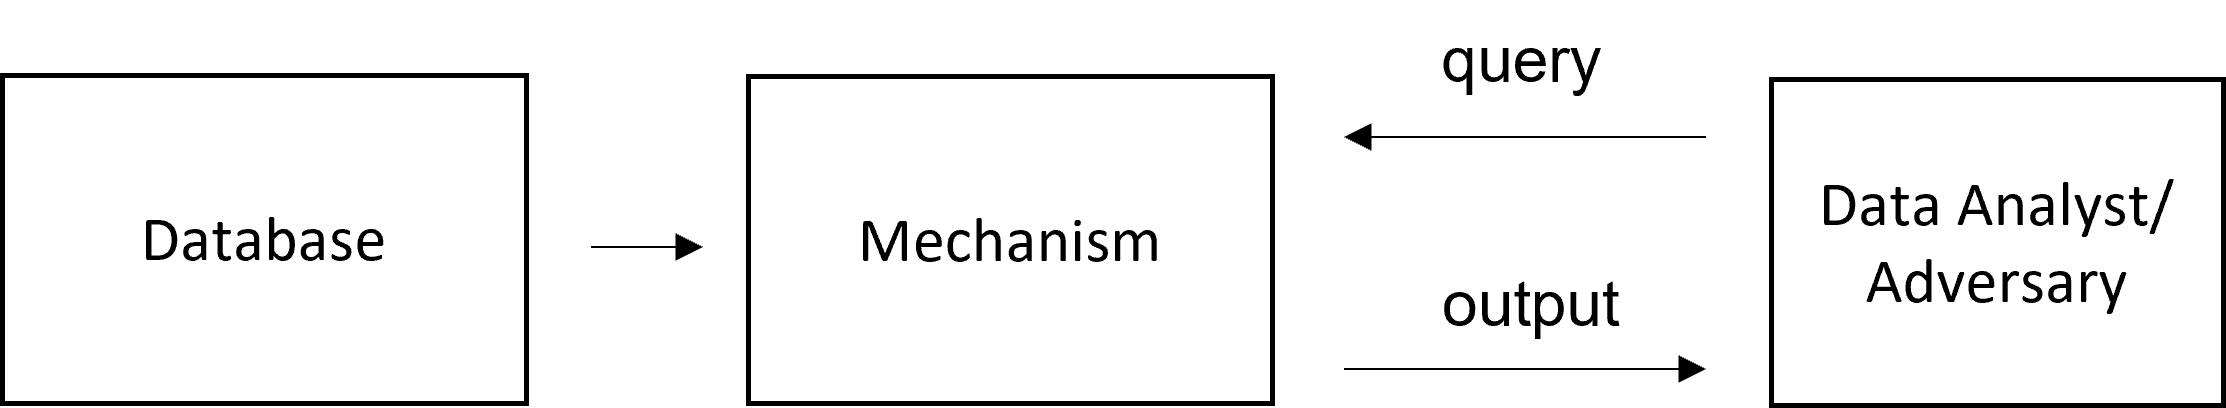
\includegraphics[width=\textwidth]{DP_setting}
    \centering
    \caption{Query process of a database.}
    \label{img:DPsetting}
\end{figure}
\FloatBarrier
% --------------------------------------------------------------------------

\begin{definition}[Neighboring Databases~\cite{dwork2014algorithmic}]
    Two databases $D_{0}$, $D_{1}\in \mathcal{X}^{n}$  are called neighboring databases if they differ in exact one entry, which is expressed as $D_{0}\sim D_{1}$.
    \label{def:NeighboringDatabases}
\end{definition}

\begin{definition}[Differential Privacy~\cite{dwork2014algorithmic}]
    A mechanism $M:\mathcal{X}^{n}\times \mathcal{Q}\rightarrow \mathcal{Y}$ is said to satisfy $\left( \varepsilon ,\delta \right)$-differential privacy if for any two neighboring databases $D_{1}$, $D_{1}\in \mathcal{X}^{n}$, and for all $T\subseteq \mathcal{Y}$,
    \[\Pr \left[ M\left( D_{0}\right) \in T\right] \leq e^{\varepsilon}\cdot \Pr \left[ M\left( D_{1}\right) \in T\right] +\delta,\]
    where the randomness is over the choices made by $M$.
    \label{def:DP}
\end{definition}
Intuitively, differential privacy implies that the output distribution of mechanism $M$ is similar for all neighboring databases. $M$ is called $\varepsilon$-\differentialprivacy (or pure \differentialprivacy) for $\delta = 0$, and $\left(\varepsilon,\delta\right)$-\differentialprivacy (or approximate \differentialprivacy) for $\delta \neq 0$.

\begin{definition}[$L_{1}$ Norm]
    The $L_{1}$ norm of a vector $\vec{X}=\left(x_1, x_2, \ldots,x_n \right)^{T}$ measures the sum of the magnitudes of the vectors $\vec{X}$ and is denoted by $\left\|\vec{X}\right\|_{1}=\sum ^{n}_{i=1}\left| x_{i}\right| $.
\end{definition}

\begin{definition}[$L_{2}$ Norm]
    The $L_{2}$ norm of a vector $\vec{X}=\left(x_1, x_2, \ldots,x_n \right)^{T}$ measures the shortest distance of $\vec{X}$ to origin point and is denoted by $\left\|\vec{X}\right\|_{2}=\sqrt{\sum ^{n}_{i=1}x_{i}^{2}}$.
\end{definition}

\begin{definition}[$\ell_{t}$-sensitivity~\cite{dwork2014algorithmic}]
    The $\ell_{t}$-sensitivity of a query function $f : \mathcal{X}^{n} \rightarrow \mathbb{R}^{k}$ is defined as $\Delta ^{\left(f\right)}_{t}=\max _{D_{0},D_{1}} \left\| f\left( D_{0}\right) -f\left( D_{1}\right) \right\| _{t}$ for $t \in \left\{1,2\right\}$, where $D_{0},D_{1}$ are neighboring databases.
    \label{def:sensitivity}
\end{definition}
Generally, the sensitivity calculates the upper bound of how much a query function $f$ can change when modifying a single entry using the notion of neighboring databases.




\subsubsection{Motivating Example of Differential Privacy}
\label{subsubsec:motivatingexampleDP}
The previous example about randomized response \autoref{subsubsection:randomizedresponse} indicates that we can use \differentialprivacy to solve the trade-off problem between learning useful statistics and preserving the individuals' privacy.
% To illustrate how \differentialprivacy solves such problems, we adapt an example from~\cite{simpleexplanDP} shown in \autoref{prot:motivationexampleDP}:
To illustrate how \differentialprivacy solves such problems, we adapt an example~\footnote{https://win-vector.com/2015/10/02/a-simpler-explanation-of-differential-privacy/} shown in \autoref{prot:motivationexampleDP}:
\begin{itemize}
    \item An adversary proposes two datasets $D_{0}$ and $D_{1}$ that differ by exactly one entry and a test set $Q$. A challenger implements a mechanism $M$ that can compute useful statistical information with databases $D_{0}$ and $D_{1}$.
    \item The challenger outputs $M\left( D_{0}\right) $, $M\left( D_{1}\right) $ to the adversary in a random order. The adversary aims to differentiate $D_{0}$ and $D_{1}$. The challenger's goal is to build a mechanism $M$ to prevent $M\left( D_{0}\right) $ and $M\left( D_{1}\right) $ from being distinguished by the adversary.
    \item Mechanism $M$ is called $\varepsilon$-\differentialprivacy iff: $\left| \frac{\Pr \left[ M\left( D_{0}\right) \in Q\right] }{\Pr \left[ M\left( D_{1}\right) \in Q \right] }\right|\leq e^{\varepsilon}$.
\end{itemize}

\begin{protocol}[tbh!]
    \centering
    \fbox{\pseudocode[space=none, syntaxhighlight=auto, addkeywords={input, output, otherwise, wins}]{%
    \textbf{Challenger $C$} \< \< \textbf{Adversary $A$} \\[0.1\baselineskip][\hline]
    \<\< \\[-0.5\baselineskip]
    \text{input: $M$} \< \< \text{input: $D_0$, $D_1$, $Q$ }\\
    \< \sendmessageleft{top={$D_0$, $D_1$}} \< \<  \\
    \text{$b \sample \bin$} \< \< \\
    \text{$M\left(D_{b}\right)$, $M\left(D_{1-b}\right)$} \< \< \\
    \< \sendmessageright{top={$M\left(D_{b}\right)$, $M\left(D_{1-b}\right)$}} \< \<  \\
    \< \< \text{$b^{\prime} \gets 0$, if $M\left(D_{1-b}\right) \in Q $} \\
    \< \< \text{$b^{\prime}\gets 1$, otherwise} \\
    \< \< \text{if $b==b^{\prime}$, $A$ wins.}
    }}
    \caption{An example of differentially private mechanism.}
    \label{prot:motivationexampleDP}
\end{protocol}
\FloatBarrier

Suppose the adversary $A$ has chosen the following databases:
\begin{itemize}
    \item $D_{0}=\left\{ 0, 0, 0,\ldots ,0\right\} $ ($100$ zeros)
    \item $D_{1}=\left\{ 1, 0, 0,\ldots ,0\right\} $ ($1$ one and $99$ zeroes).
\end{itemize}

The test set $Q$ is an interval $\left[ T,1\right] $ with a threshold $T$. After choosing the threshold $T$, the adversary output $b^{\prime} \gets 0$ when $T<M\left( D_{1-b}\right) < 1$, or $b^{\prime} \gets 1$ when $0<M\left( D_{1-b}\right) \leq T$. The adversary's goal is to find a \textit{good} threshold $T$ that helps him output a $b^{\prime}$ that equals $b$ with high probability and win the game.

\textbf{The Deterministic Case.}
Suppose mechanism $M$ compute the mean value of the given databases $D_0$ and $D_1$, where $M\left( D_{0}\right) =0$ and $M\left( D_{1}\right) =0.01$. The adversary can set the test set $Q =\left[ 0.005,1\right] $ win every game. In \autoref{img:DPexamplenoisefree}, the blue line represents the value of $M\left( D_{0}\right)$, whereas the orange line represents the value of $M\left( D_{1}\right)$ (plotted upside down for clarity). The vertical dotted line is the threshold $T=0.005$ that separates $D_{0}$ and $D_{1}$ correctly.

\begin{figure}[htbp]
    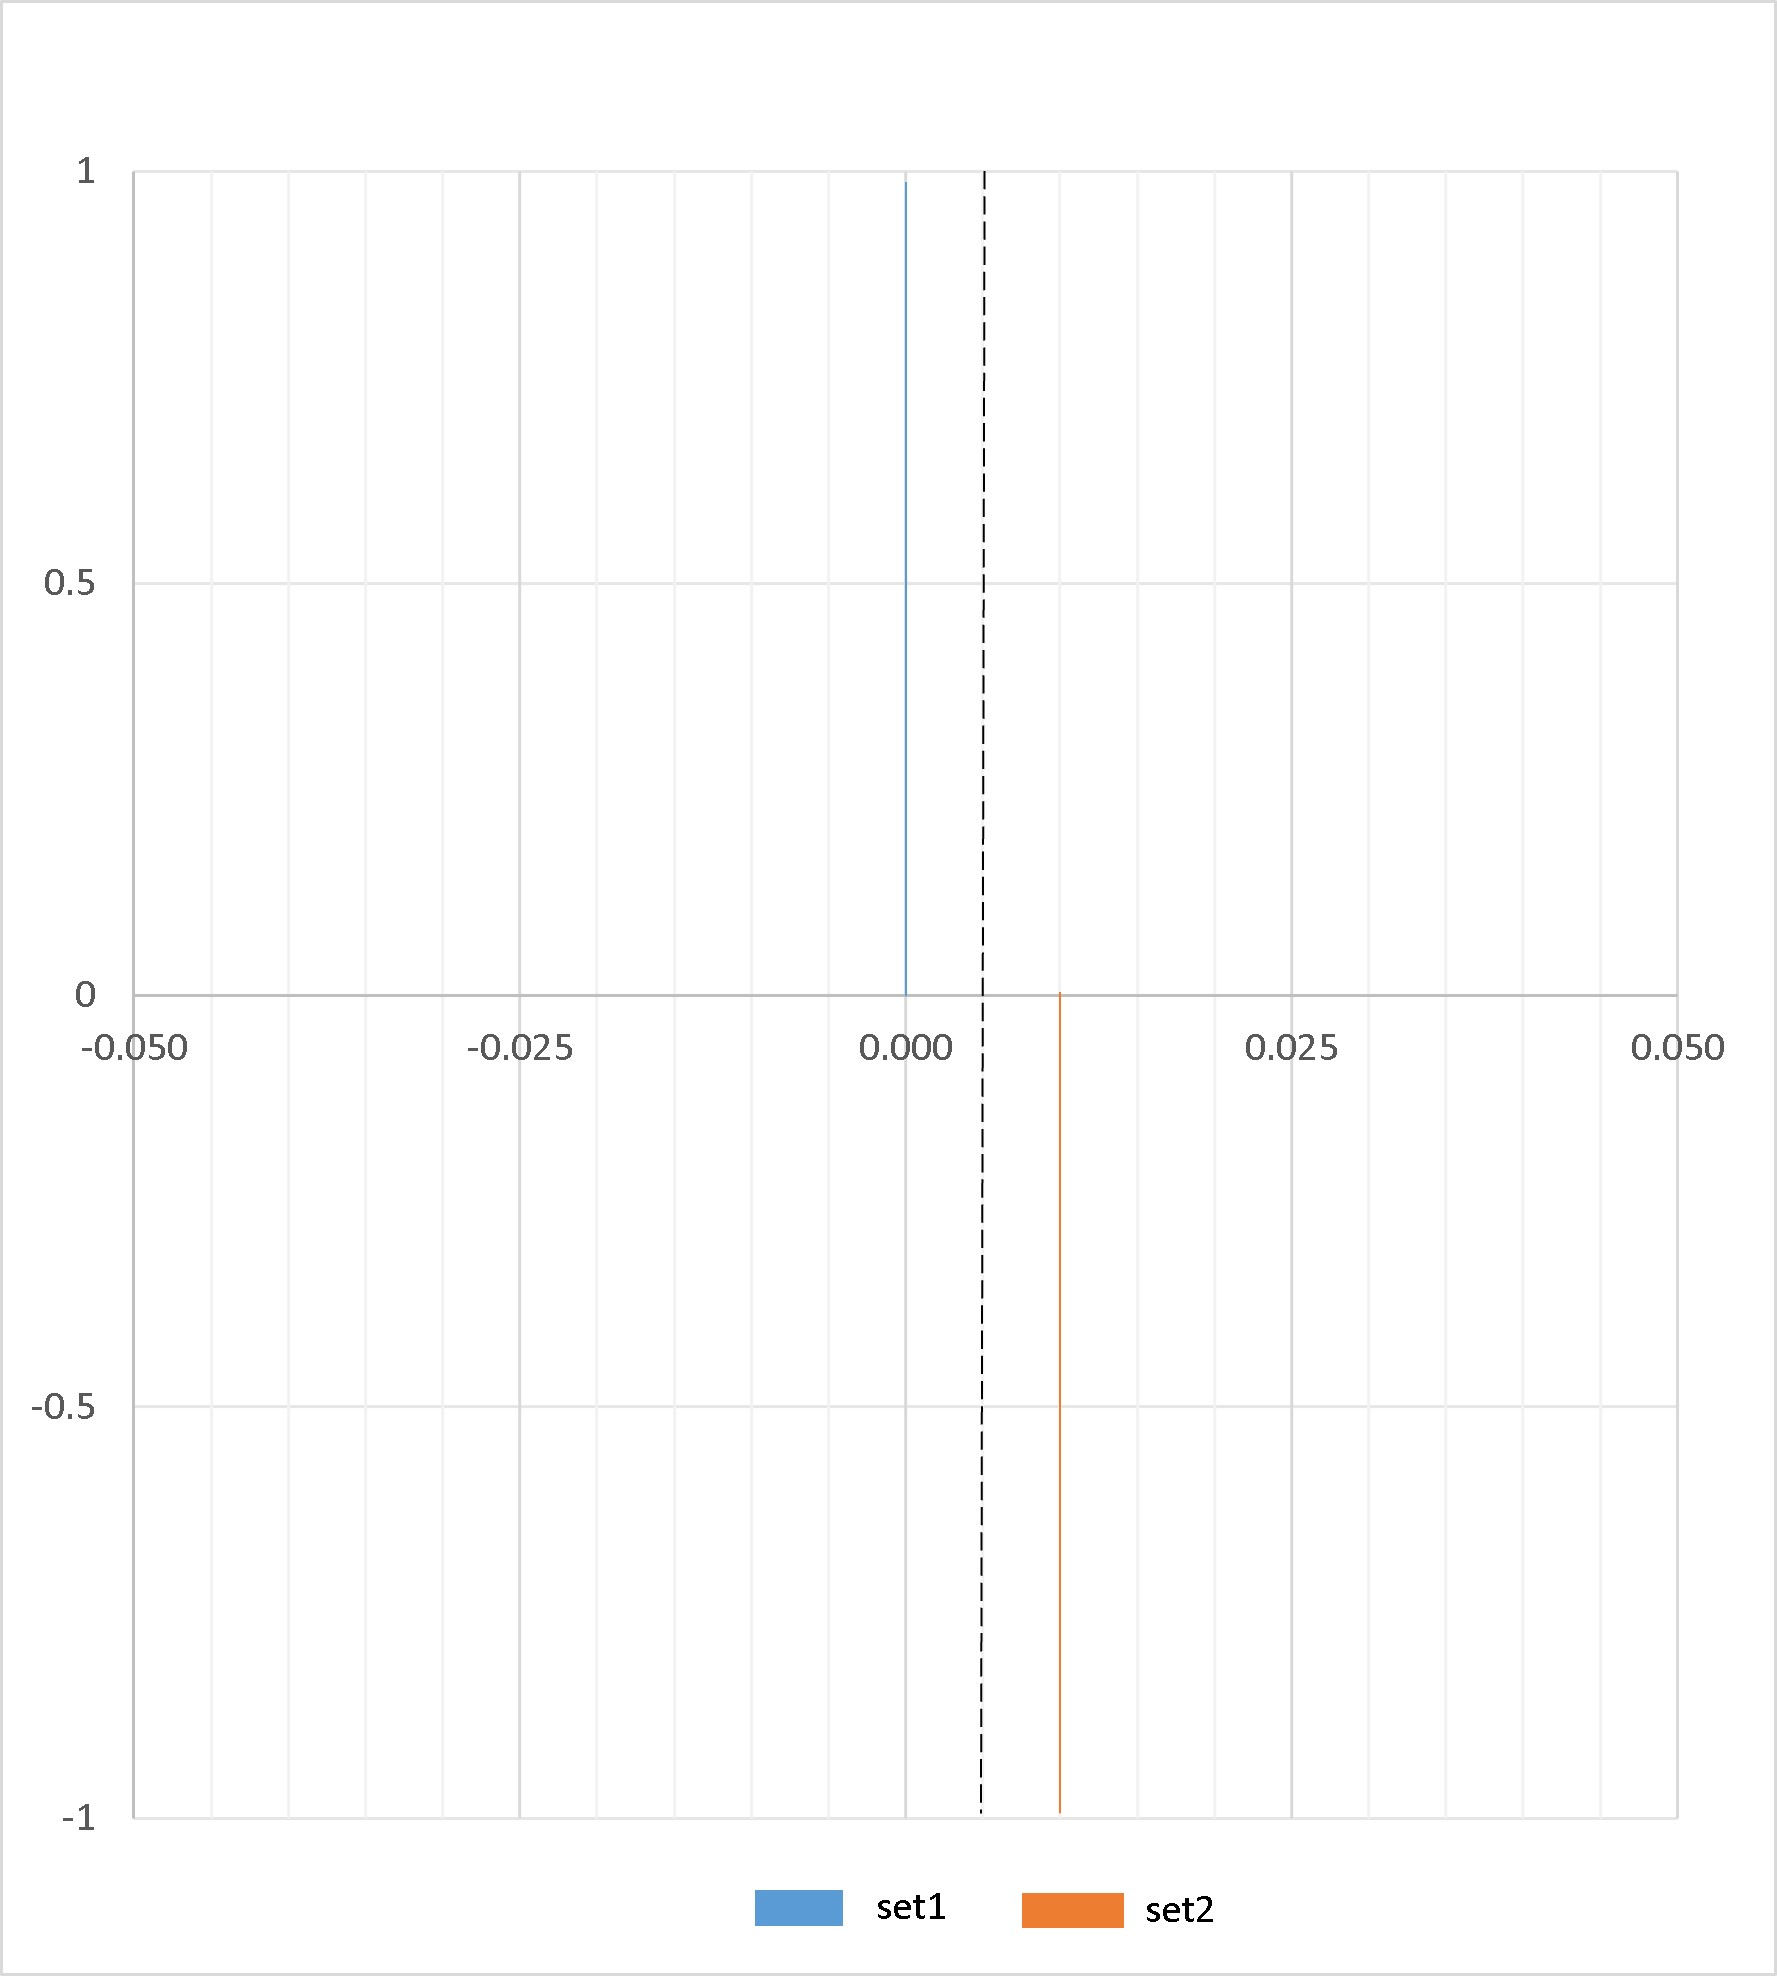
\includegraphics[width=8cm]{DPexamplenoisefree}
    \centering
    \caption{Deterministic algorithm.}
    \label{img:DPexamplenoisefree}
\end{figure}
\FloatBarrier

\textbf{The Indeterministic Case.}
The challenger takes some measures to \textit{blur} the outputs of $M\left( D_{0}\right)$ and $M\left( D_{1}\right)$ and make them hard to differentiate. Suppose the challenger decides to add the Laplace noise $lap\sim Laplace\left(b=0.05\right)$ to the result of $M\left(D\right)$ as \autoref{img:DPexamplesmallnoise} shows. The shaded blue region is the probability that $M\left( D_{0}\right)$ returns a value greater than the threshold $T$, and the adversary mistakes $D_{0}$ for $D_{1}$. In contrast, the shaded orange area is the probability that the adversary identify $D_{1}$ successfully. The challenger can decrease the adversary's success probability by adding stronger noise as \autoref{img:DPexamplelargenoise} shows, where the shaded blue and orange areas are almost of the same size. In fact, we have $\varepsilon=\left\lvert \ln \left( \frac{\textit{blue area}}{\textit{orange area}}\right)\right\rvert  $, where $\varepsilon$ describes the degree of differential privacy. A smaller $\varepsilon$ indicates a stronger privacy protection. Note that the challenger can add more noise to decrease the adversary's success probability, but the accuracy of the mean estimation decreases.


% \TODO{need reproduce following figures}
\begin{figure}[htbp]
    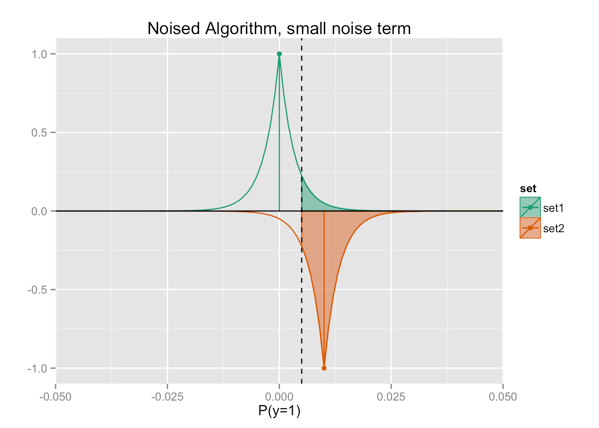
\includegraphics[width=8cm]{DPexamplesmallnoise}
    \centering
    \caption{Indeterministic algorithm with small noise ($b=0.005$).}
    \label{img:DPexamplesmallnoise}
\end{figure}
\FloatBarrier

\begin{figure}[htbp]
    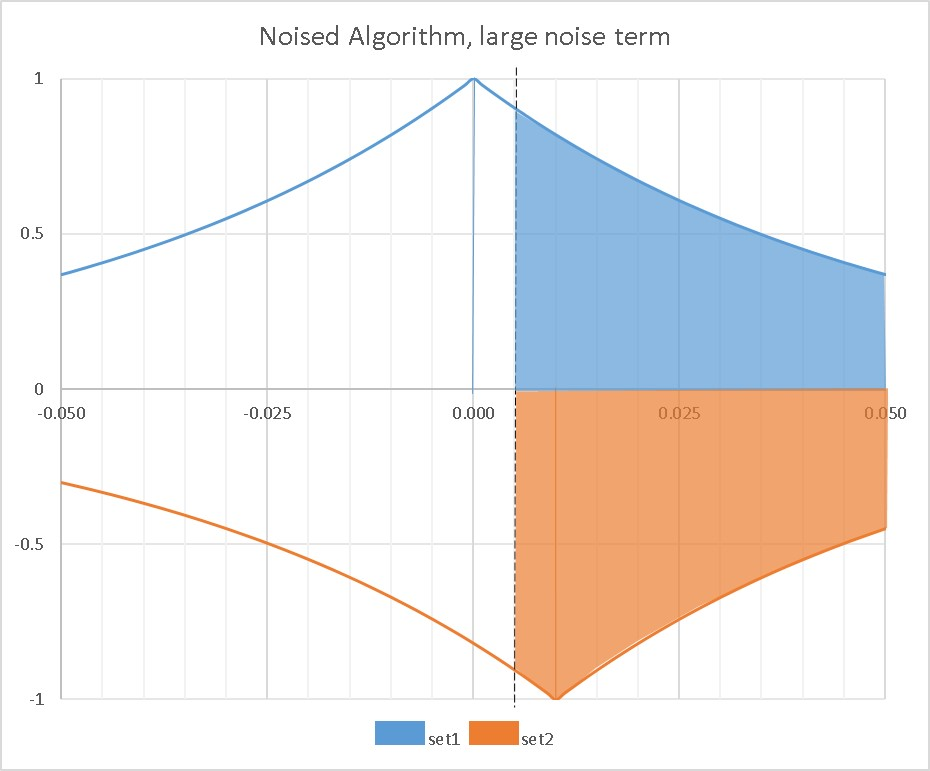
\includegraphics[width=8cm]{DPexamplelargenoise}
    \centering
    \caption{Indeterministic algorithm with large noise ($b=0.05$).}
    \label{img:DPexamplelargenoise}
\end{figure}
\FloatBarrier

\subsubsection{Differentially Private Mechanisms}
\label{subsubsec:DPMechanisms}

Differential privacy is a formal framework to quantify the trade-off between privacy and the accuracy of query results. In this part, we introduce two common differentially private mechanisms.

% \paragraph{$\varepsilon$-Differential Privacy}
\begin{definition}[Laplace Mechanism~\cite{dwork2014algorithmic}]\
    \label{def:laplaceMechanism}
    Let $f : \mathcal{X}^{n} \rightarrow \mathbb{R}^{k}$. The Laplace mechanism is defined as $M_{Lap}\left( X\right) =f\left( X\right) +\left( Y_{1},\ldots ,Y_{k}\right) $, where the $Y_{i}$ are independent Laplace random variables drawn from a Laplace distribution $Lap \left(  Y_{i}\,|\, b\right) =\frac{1}{2b}e^{\left( -\frac{\left  | Y_{i}\right|}{b}\right)} $ with $b=\frac{\Delta _{1}^{\left(f\right)}}{\varepsilon }$.
\end{definition}

\begin{theorem}
    The Laplace Mechanism satisfies $\varepsilon$-\differentialprivacy~\cite{dwork2014algorithmic}.
\end{theorem}

\begin{definition}[Gaussian Mechanism~\cite{dwork2014algorithmic}]
    Let $f : \mathcal{X}^{n} \rightarrow \mathbb{R}^{k}$. The Gaussian mechanism is defined as $M\left( X\right) =f\left( X\right) +\left( Y_{1},\ldots ,Y_{k}\right) $, where the $Y_{i}$ are independent Gaussian random variables drawn from a Gaussian distribution $\mathcal{N}  \left(  Y_{i}\,|\, \mu ,\sigma ^{2}\right) =\frac{1}{\sigma \sqrt{2\pi }}e^{-\frac{1}{2}\left( \frac{Y_{i}-\mu}{\sigma }\right) ^{2}}$ with  $\mu=0$, $\sigma ^{2}=2\cdot \ln \left( \frac{1.25}{\delta }\cdot \left( \frac{ \Delta _{2}^{\left(f\right)}) ^{2}}{\varepsilon ^{2}}\right) \right)$ .
    \label{def:gaussianMechanism}
\end{definition}

\begin{theorem}
    The Gaussian mechanism satisfies $\left(\varepsilon,\delta\right)$-\differentialprivacy~\cite{dwork2014algorithmic}.
\end{theorem}

\subsubsection{Properties of Differential Privacy}
We introduce three fundamental properties of \differentialprivacy~\cite{dwork2006differential, dwork2006calibrating} based on work~\cite{dwork2014algorithmic}.

% \paragraph{Post-Processing}
\begin{prop}[\textbf{Post-Processing}] Let $M:\mathcal{X}^{n} \rightarrow \mathcal{Y}$ be a $\left(\varepsilon,\delta \right)  $-\differentialprivacy mechanism, and let $F:\mathcal{Y}\rightarrow \mathcal{Z}$ be an arbitrary randomized mapping. Then $F\circ M$ is $\left(\varepsilon,\delta\right)  $-DP.
    \label{prop:Post-Processing}
\end{prop}
The post-processing property implies that once a database is privatized, it is also differentially private after further processing.

% \paragraph{Group Privacy}
\begin{prop}[\textbf{Group Privacy}] Let $M:\mathcal{X}^{n} \rightarrow \mathcal{Y}$ be a $\left( \varepsilon ,\delta \right)$-\differentialprivacy mechanism. For all $T\subseteq \mathcal{Y}$,
    \[\Pr \left[ M\left(D_{0}\right) +T\right] \leq e^{k \varepsilon}\cdot \Pr \left[ M\left( D_{1}\right) \in T\right] +\delta, \]
    where $D_{0}$, $D_{1}\in \mathcal{X}^{n}$ are databases that differ in exactly $k$ entries.
\end{prop}

The group privacy property indicates that \differentialprivacy can also be extended to the case when two databases have more than one entry difference. However, as $k$ increases, the privacy decay rate $e^{k\varepsilon}$ also increases, which implies a weaker level of privacy protection.

% \paragraph{Basic Composition}
\begin{prop}[\textbf{Basic Composition}]
    Suppose $M=\left( M_{1}\ldots M_{k}\right)$  is a sequence of $\left( \varepsilon_{i} ,\delta_{i} \right)$-\differentialprivacy mechanisms, where $M_{i}$ is chosen sequentially and adaptively. Then, $M$ is $\left(\sum_{i=1}^n\varepsilon_{i} ,\sum_{i=1}^n\delta_{i} \right)$-\differentialprivacy.
\end{prop}

The basic composition property provides a way to evaluate the overall privacy guarantee of the released result when $k$ differentially private mechanisms are applied to the same dataset.

% \subsection{Comparison between Differential Private Mechanisms}


% \begin{proof}
%     Let $D_{0}$ and $D_{1}$ be any two neighbouring databases that differs in one entry. Let $\Pr_{D_{0}}\left(z\right) $ and $\Pr_{D_{1}}\left( z\right) $ be the probability density functions of $M\left( D_{0}\right) $ and $M\left( D_{1}\right) $ evaluated at a point $z \in \mathbb{R}^{k}$. To prove differential privacy, it necessary to show that the ratio $\frac{\Pr_{D_{0}}\left( z\right) }{\Pr_{D_{1}}\left( z\right) }$ is bounded by $\varepsilon$, for any arbitrary $z$ and neighboring $D_{0}$ and $D_{1}$ .

%     \begin{align*}
%         \frac{\Pr_{D_{0}}\left( z\right) }{\Pr_{D_{1}}\left( z\right) } & =\frac{ \prod _{i=1}^{k}\exp{\left( -\frac{ \varepsilon \left| f\left( D_{0}\right) _{i}-z_{i} \right|}{\Delta }\right) }}{\prod_{i=1}^{k}\exp{\left( -\frac{ \varepsilon \left| f\left( D_{1}\right) _{i}-z_{i} \right|}{\Delta }\right) } } \\
%                                                                         & =\prod_{i=1}^{k} \exp \left(-\frac{\varepsilon\left(\left|f(D_{0})_{i}-z_{i}\right|-\left|f(D_{1})_{i}-z_{i}\right|\right)}{\Delta}\right)                                                                                                    \\
%                                                                         & \leq \prod_{i=1}^{k} \exp \left(\frac{\varepsilon\left|f(D_{1})_{i}-f(D_{0})_{i}\right|}{\Delta}\right)                                                                                                                                       \\
%                                                                         & =\exp \left(\frac{\varepsilon \sum_{i=1}^{k}\left|f(D_{1})_{i}-f(D_{0})_{i}\right|}{\Delta}\right)                                                                                                                                            \\
%                                                                         & =\exp \left(\frac{\varepsilon\|f(D_{1})-f(D_{0})\|_{1}}{\Delta}\right)                                                                                                                                                                        \\
%                                                                         & \leq \exp (\varepsilon).                                                                                                                                                                                                                      \\
%     \end{align*}
% \end{proof}

% \begin{definition}[Privacy Loss~\cite{dwork2014algorithmic}]
%     Let $X$ and $Y$ be two random variables. The privacy loss random variable  $\mathcal{L}_{X||Y}$ is distributed by drawing $t \sim Y$ , and outputting $\ln ( \frac {\Pr \left[ X=t\right] )}{\Pr \left[ Y=t\right] )} $.
% \end{definition}

% The definition of \emph{Privacy Loss} relies on the assumption that the supports of $X$ and $Y$ are equal, where $supp\left(f\right)=\left\{x \in X: f\left(x\right) \neq 0\right\}$. Otherwise, the privacy loss is undefined since $\Pr\left\{Y=t\right\}=0$.

% From the definition of $\varepsilon$-DP, it is not difficult to see that $\varepsilon$-DP corresponds to $\left|\mathcal{L}_{D_{0}||D_{1}}\right|$ being bounded by $\varepsilon$ for all neighboring databases $D_{0}$, $D_{1}$. In other words, $\varepsilon$-DP says that the absolute value of the privacy loss random variable is bounded by $\varepsilon$ with probability 1.

% \paragraph{$\left(\varepsilon,\delta\right)$-Differential Privacy}
% $\varepsilon$-DP has strong privacy requirement which leads to adding too much noise and affecting the accuracy of the queries. We introduce an relaxation of $\varepsilon$-DP, $\left(\varepsilon,\delta\right)$-DP.




% \subsubsection{Discussion about Differential Privacy}

% \paragraph{Local and Central Differential Privacy.}
% Differential privacy is a definition that can be realized in many ways. Two common modes of DP are centralized differential privacy~\cite{dwork2014algorithmic} and local differential privacy~\cite{dinur2003revealing}.

% In centralized DP, all data is stored centrally and managed by a trusted curator before the differentially private mechanism is applied. As \autoref{img:DPcentral} shows, the raw data from clients is first collected in a centralized database, then, the curator applies the privacy mechanism and answers the queries $f\left(x\right)$ with $f^{\prime}\left(x\right)$.
% The local DP mode is, as \autoref{img:DPlocal} shows, where the clients first apply a privacy mechanism on their data, and send the perturbed data to the curator.
% An advantage of local DP mode is that no trusted central curator is needed since the data is perturbed independently before sending to the curator. However, the disadvantage is that the collected data contains redundant noise and may decrease the utility.

% \TODO{reproduce following figures}
% \begin{figure}[htbp]
%     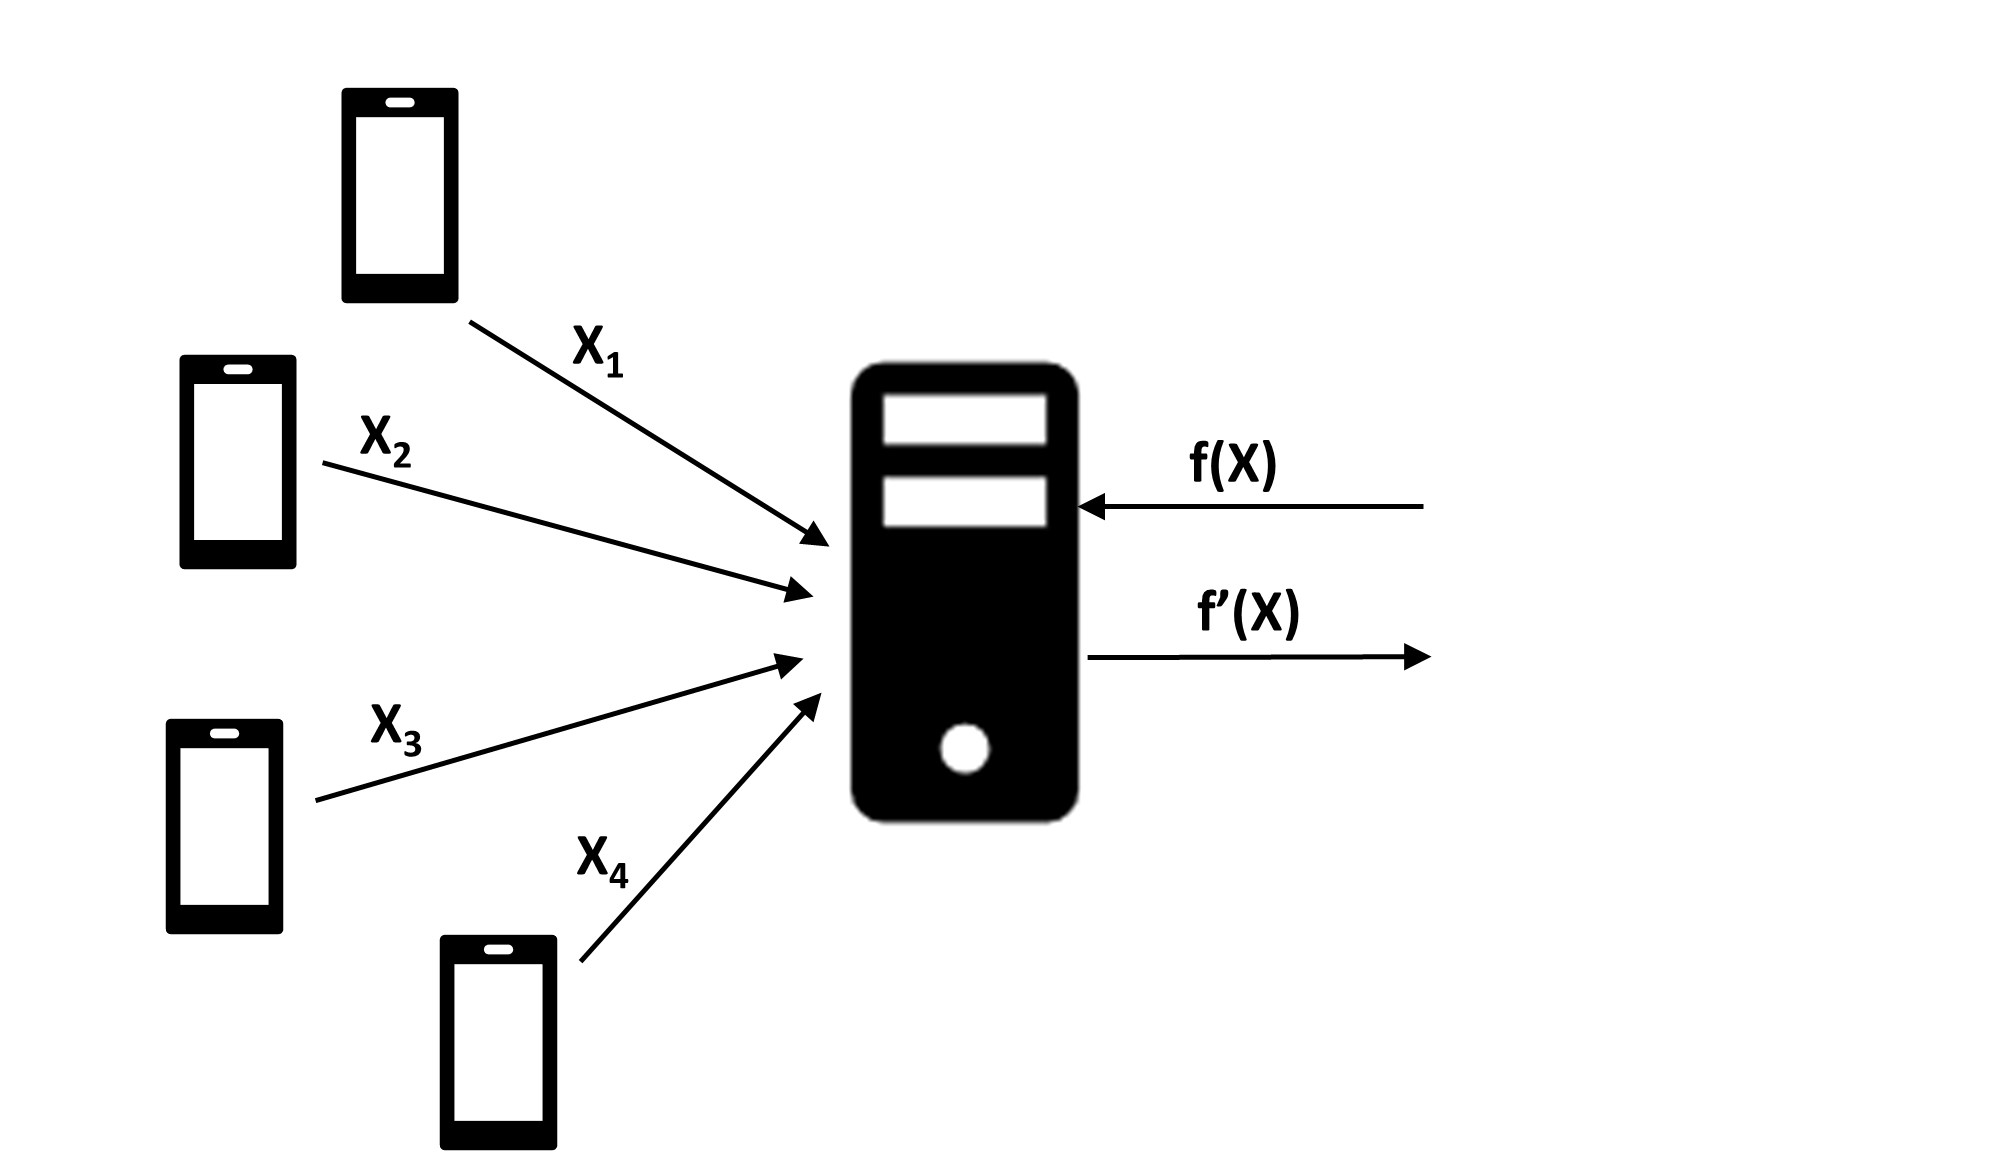
\includegraphics[width=10cm]{DPcentral}
%     \centering
%     \caption{Centralized DP mode.}
%     \label{img:DPcentral}
% \end{figure}
% \FloatBarrier

% \begin{figure}[htbp]
%     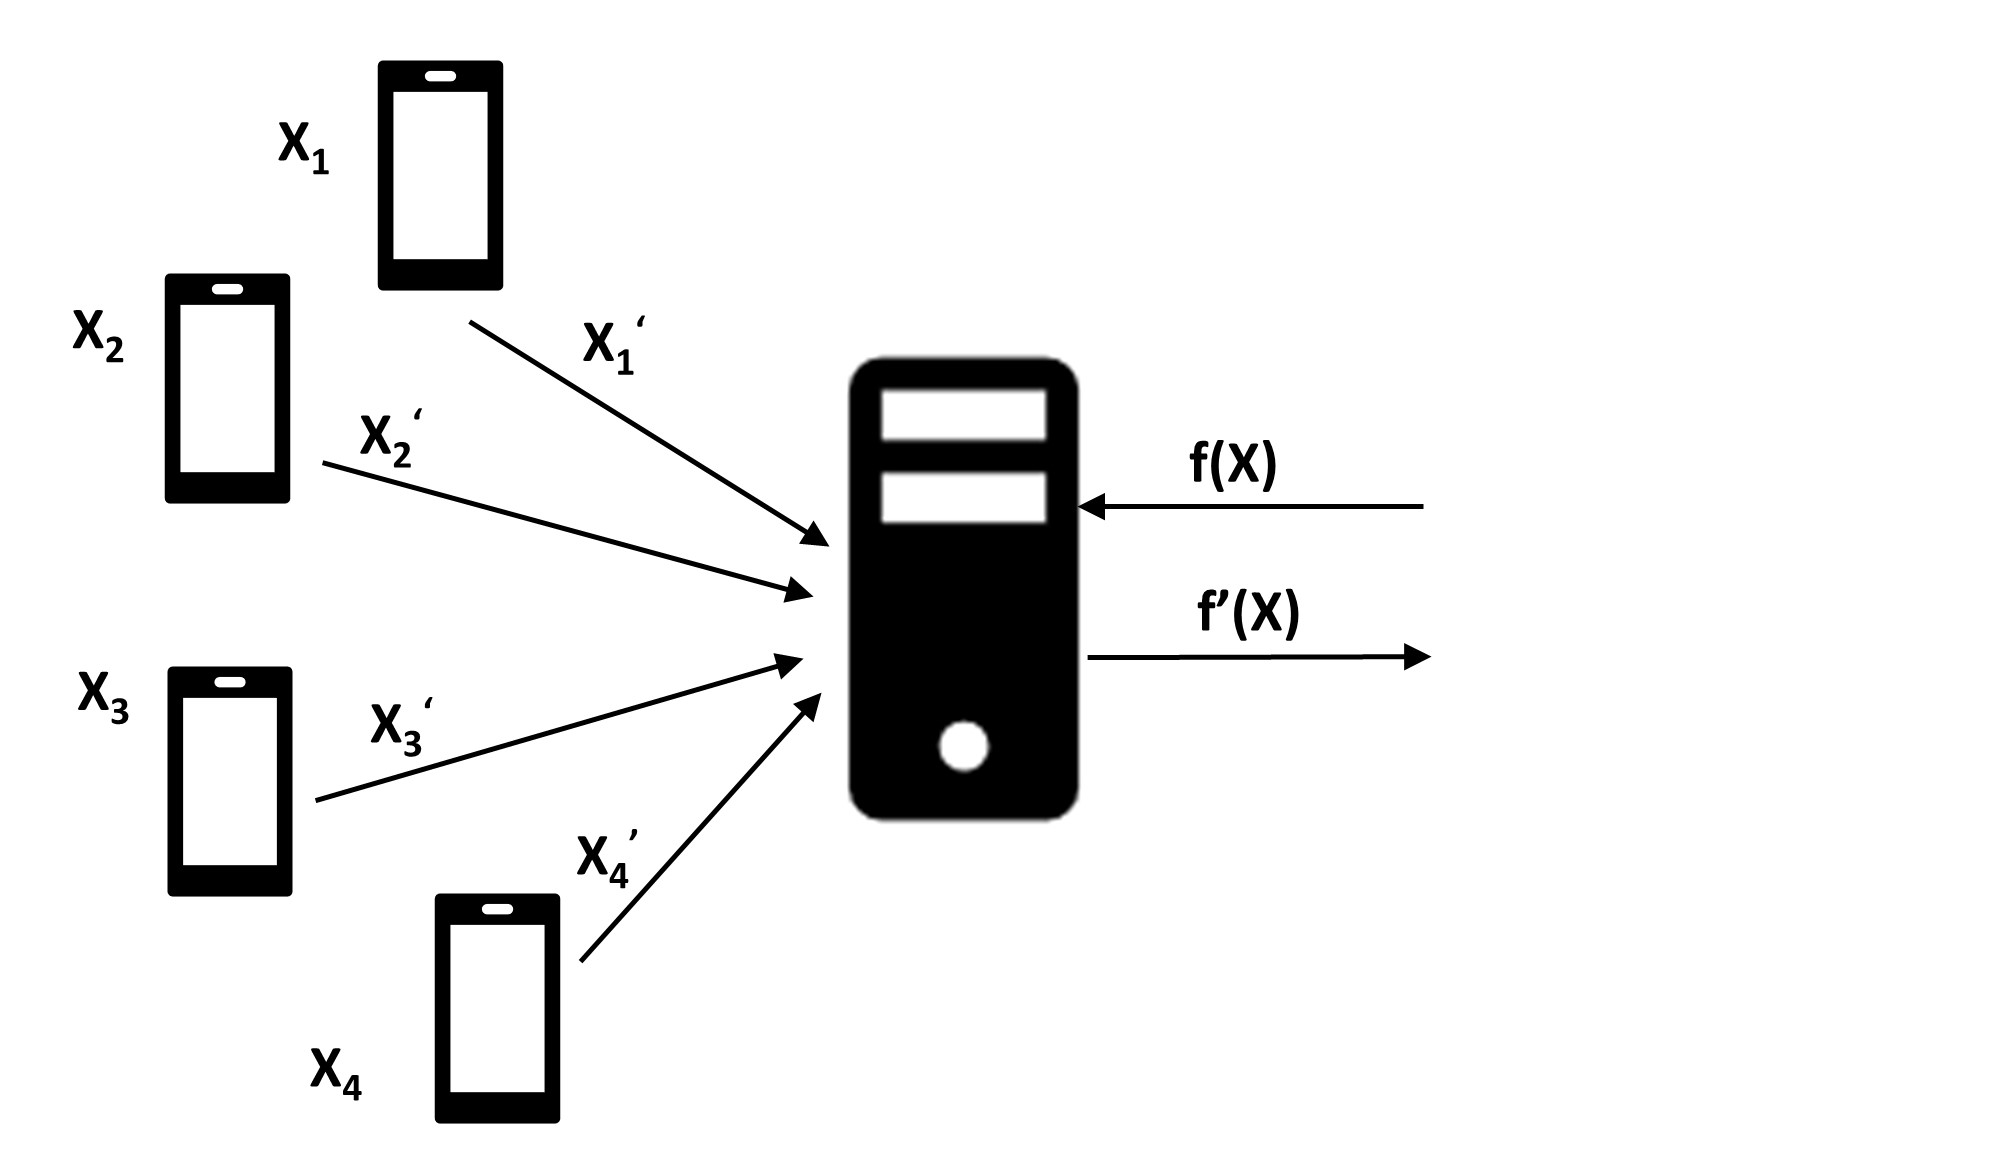
\includegraphics[width=10cm]{DPlocal}
%     \centering
%     \caption{Local DP mode.}
%     \label{img:DPlocal}
% \end{figure}
% \FloatBarrier


% \paragraph{Advantages of Differential Privacy}
% From the example \autoref{subsubsec:motivatingexampleDP}, we found that DP can still protect privacy even if the adversary has the knowledge of the database. Generally speaking, DP ensures privacy protection by making no assumption about the adversary's auxiliary information (even when the adversary is the data provider) or computational strategy (regarding the complexity of modern cryptography)~\cite{vadhan2017complexity}. In addition, DP provides a quantitive theory about safely releasing data and maintaining certain level of accuracy.

\subsubsection{Challenges of Differential Privacy}
\label{subsubsec:challengesOfDP}
Differential privacy provides a method to guarantee and quantify individual privacy at the theoretical level. However, it faces a series of challenges in practical application scenarios.

\paragraph{Sensitivity Calculation.}
As discussed in~\autoref{subsubsec:DPMechanisms}, we first need to compute or estimate the sensitivity of the query function before applying differentially private mechanism. Take a database with human ages as an example, the ages should be bounded in the interval $\left[0,150\right] $ (the longest human lifespan is $122$ years and $164$ days according to~\cite{whitney_1997}). However, the data with an unbounded value range brings great challenges. A common solution is to roughly estimate a \textit{reasonable} value range and limit the data within that range. If the value range is chosen too wide (i.e., a larger sensitivity estimation), the differentially private mechanism applies too strong noise to perturb the data, and the utility of the result might be destroyed. Nevertheless, a narrow value range estimation may also decrease the utility as too much data beyond the value range is discarded.

\paragraph{Security Issue in the Practical Implementation.}
\label{para:SecurityIssueinthePracticalImplementation}
Generally, the security analysis of differentially private mechanisms is based on two implicit assumptions: (i) Computations are performed on real numbers and require machines to have infinite precision, (ii) The noise is sampled from a probability distribution that is very close to the theoretically correct probability distribution.
However, the practical implementation of differentially private mechanisms is typically based on floating-point or fixed-point arithmetic that only provides finite order of accuracy.
Mironov~\cite{mironov2012significance} demonstrated that the Laplace random noise sampled with textbook algorithm (cf.~\autoref{algo:InverseTransform-BasedLaplaceSamplingMethod}) under floating-point implementation could lead to violation of differential privacy.
Specifically, for database $D$ and a Laplace Mechanism $M$ that samples the Laplace noise with the methods introduced in~\autoref{algo:InverseTransform-BasedLaplaceSamplingMethod}, $M\left(D\right) $ fails to output certain floating-point numbers that can be related to database $D$. By comparing the missed out floating-point numbers, an adversary can differentiate between database $D$ and its neighboring database $D^{\prime}$ even extract the entire content of database $D$.
Based on the similar vulnerability of floating-point numbers, Jin et al.~\cite{jin2022we} presented a series of floating-point attacks against the Gaussian noise sampling algorithms. In addition, they also constructed a timing attack against the discrete noise sampling algorithms, i.e., the magnitude of the discrete noise can be predicted by measuring the sampling time.
Gazeau et al.~\cite{gazeau2016preserving} proved that any differentially private mechanisms perturb data by adding noise with a finite precision could lead to secret disclosure regardless of the actual implementation.
This work aims to realize differentially private mechanisms with secure noise generation methods in \smpc that are free of the above attacks.

% The theory of \differentialprivacy is built upon the real number arithmetic. The practical implementation of differentially private mechanisms relies on floating-point or fixed-point arithmetic only provides an approximation of the mathematical abstractions. Mironov~\cite{mironov2012significance} showed that the irregularities of floating-point implementations and porous distribution of the Laplace mechanism with textbook sampling algorithm lead to the breach of differential privacy. Further, 

% -------------------------------------------------------------


% Similar to $\varepsilon$-DP, $\left(\varepsilon,\delta\right)$-DP can also be interpreted regarding privacy loss: the absolute value of the privacy loss random variable is bounded by $\varepsilon$ with probability $1 - \delta$~\cite[Lemma 3.17]{dwork2014algorithmic}. In other words, with probability $ \delta$, the privacy of databases is breached.
